\subsection{零化子。忠实模。单生成模。}

定义11. A模E的子集S的零化子是所有满足下列条件的元素 \(\alpha \in \mathbf{A}\) 组成的集合：\(\alpha x = 0\) 对所有 \(x \in S\) 成立.

S 的零化子通常记为 Ann(S)；对于由单个元素 x 组成的子集 S，我们写 Ann(x) 而不写 Ann(\{x\})，并把 Ann(x) 称为 x 的零化子。

关系 \(\alpha x = 0\) 也可以说成： \(x\) 被 \(\alpha\) 零化.

立即可以看出，E的任意子集S的零化子是A的一个左理想；要使它等于A，必须且只需（根据 \((\mathbf{M}_{\mathrm{IV}})\) ）有 \(S = \{0\}\) 。如果 E 的两个子集 S、T 满足 \(S \subset T\) ，则 T 的零化子包含于 S 的零化子中。如果 \((\mathbf{S}_{t})_{t \in I}\) 是E的任意子集族，则并集 \(\bigcup_{t} S_{t}\) 的零化子是诸 \(S_{t}\) 的零化子的交。特别地，E 的子集 S 的零化子是 S 中各元素的零化子的交。说 E 的一个元素是自由的，等价于说它的零化子是 \(\{0\}\) 。对所有 \(x \in E\) 以及所有 \(\alpha \in A\) ， \(\alpha x\) 的零化子是这样的 \(\beta \in A\) 组成的集合，使得 \(\beta \alpha \in \text{Ann}(x)\) .

子模M在E中的零化子是A的一个双边理想；因为，若 \(\alpha x = 0\) 对所有 \(x \in M\) 成立，则 \(\alpha(\beta x) = 0\) 也对所有 \(x \in M\) 以及所有 \(\beta \in A\) 成立，因此 \(\alpha\beta\) 对所有 \(\beta \in A\) 都属于M的零化子。特别地，E的零化子是A的一个双边理想。

对于所有 \(\alpha \in \mathbf{A}\) ，设 \(h_{\alpha}\) 为位似变换 \(x \mapsto \alpha x\) ；已知映射 \(\alpha \mapsto h_{\alpha}\) （从 \(\mathbf{A}\) 到自同态环 \(\mathcal{E} = \operatorname{Hom}_{\mathbf{Z}}(\mathbf{E}, \mathbf{E})\) ，即无算子的交换群 \(\mathbf{E}\) 的自同态环）是一个环同态（ \(\S 2\) ，第5号）。该同态下0的原像是零化子 \(\mathfrak{a}\) （即 \(\mathbf{E}\) 的零化子）；因此， \(\mathbf{A}\) 在同态 \(\alpha \mapsto h_{\alpha}\) 下的像同构于商环 \(\mathbf{A}/\mathfrak{a}\) 。模 \(\mathbf{E}\) 称为忠实的，如果其零化子 \(\mathfrak{a}\) 缩减为0。

设 E 为任意 A-模，a 为 A 中包含于 Ann(E) 的一个双边理想，并设 \(\dot{\alpha}\) 为商环 A/a 的一个元素；对所有 \(x \in E\) ，元素 \(\alpha x\) 只依赖于 \(\alpha \in A\) 所属的类 \(\dot{\alpha} \mod a\) ；若将此元素记为 \(\dot{\alpha}x\) ，则立即可以看出，映射 \((\dot{\alpha}, x) \mapsto \dot{\alpha}x\) （连同 E 上的加法）在 E 上定义了一个 (A/a)-模结构。当 \(a = \text{Ann}(E)\) 时，如此定义的 (A/a)-模 E 是忠实的；我们称它为与 A-模 E 相伴的忠实模。注意，A-模 E 的每个子模也是相伴忠实模的子模，反之亦然。

定义12. 一个模称为单生成的，如果它由单个元素生成。

第7号命题9表明，如果E是一个单生成A-模且a是生成E的元素，则E与集合A.a 相同，它由 \(\xi a\) 组成，其中 \(\xi\) 遍历A。

例. (1) 每个单生成群，由于是交换的（I，§ 4，第10号，命题18），都是一个单生成Z-模。

\begin{enumerate}
\def\labelenumi{(\arabic{enumi})}
\setcounter{enumi}{1}
\item
  若A是交换环，则A-模A的单生成子模恰好就是环A的主理想（I，§ 8，第6号）。
\item
  每个单A-模E是单生成的，因为由E中元素 \(\neq0\) 生成的E的子模必然等于E。
\end{enumerate}

命题22. 设 A 为一个环。 \(\mathbf{A}_s\) 的每个商模都是单生成的。反之，设 E 为一个单生成 A-模， \(c\) 为 E 的一个生成元，a 为其零化子；线性映射 \(\xi \mapsto \xi c\) 在过渡到商后定义了 \(\mathbf{A}_s / \mathfrak{a}\) 到 E 上的一个同构。

由于 \(A_{s}\) 本身是单生成的（由 1 生成），第一个断言由第7号命题9的推论1得出。第二个断言是显然的，因为 \(\xi \mapsto \xi c\) 根据假设是满射的且核为 a。

注意，若 A 非交换，则单生成 A-模 E 的两个不同生成元 c, \(c'\) 的零化子一般互不相同，并且也与模 E 的零化子不同。另一方面，若 A 是交换的，则 E 的一个生成元 c 的零化子包含于 E 的每个元素的零化子之中，因此就是整个 E 的零化子。

推论。单生成A-模E的每个子模都同构于一个商模b/a，其中a和b是A的两个左理想，使得 \(a \subset b\) 。单生成A-模的每个商模都是单生成的。

第二个断言是显然的，第一个断言由命题22及I，§4，第6号，定理4得出。

另一方面，请注意，单生成模的子模不一定是单生成的。例如，若A是一个存在非主理想的交换环（VII，§1，第1号），则这些理想是单生成A-模A的非单生成子模。

由定义可知，A-模E的由E中元素族 \((a_{t})\) 生成的子模是诸单生成子模

\(Aa_{t}\) 之和；要使 \((a_{t})\) 成为E的一组基，必须且只需每一个 \(a_{t}\) 都是E的自由元素，并且诸 \(Aa_{t}\) 的和是直和。

命题23. 设E是一个A-模，它是一族无限多个非零子模 \((\mathbf{M}_t)_{t\in I}\) 的直和。对于E的每一个生成系S， \(\operatorname{Card}(\mathbf{S})\geqslant \operatorname{Card}(\mathbf{I})\)

对于所有 \(x \in S\) ，设 \(C_x\) 为指标 \(i \in I\) 组成的有限集，使得 \(x\) 在 \(M_i\) 中的分量 \(\neq 0\) ，并设 \(C = \bigcup_{x \in S} C_x\) 。每个 \(x \in S\) 按定义属于 \(E\) 的由诸 \(M_i\) （ \(i \in C\) ）组成的直和子模，且 \(S\) 生成 \(E\) 这一假设因此蕴含 \(C = I\) ；由于 \(I\) 按假设是无限的， \(S\) 也是无限的（集合论，III，§5，第1号，命题1的推论1）；因此 \(\text{Card}(I) = \text{Card}(C) \leqslant \text{Card}(S)\) （集合论，III，§6，第3号，定理2的推论3）。

推论1. 在命题23的假设下，再设每个 \(\mathbf{M}_{\iota}\) 都是单生成的，且 \(\mathbf{E}\) 是第二个由非零单生成子模组成的族 \((\mathrm{N}_{\lambda})_{\lambda \in \mathbf{L}}\) 的直和。则 \(\operatorname{Card}(\mathbf{L}) = \operatorname{Card}(\mathbf{I})\) .

若 \(b_{\lambda}\) 是 \(\mathbf{N}_{\lambda}\) 的一个生成元，则诸 \(b_{\lambda}\) 组成的集合是 \(\mathbf{E}\) 的一个生成系，因此 \(\operatorname{Card}(\mathbf{L}) \geqslant \operatorname{Card}(\mathbf{I})\) 。特别地， \(\mathbf{L}\) 是无限的，并且交换 \((\mathbf{M}_i)\) 与 \((\mathbf{N}_{\lambda})\) 的角色，类似地有 \(\operatorname{Card}(\mathbf{I}) \geqslant \operatorname{Card}(\mathbf{L})\) ，由此得出推论。

推论2. 若模E具有无限基B，则E的每个生成系的基数 \(\geqslant\) Card(B)，且E的每个基都与B等势。

\subsection{标量环的更换}

设 A、B 为两个环，且 \(\rho\) 为从环B到环A的一个同态。对于每个A-模E，外合成律 \((\beta, x) \mapsto \rho(\beta)x\) （连同加法）定义了一个B-模结构，称为与 \(\rho\) 及E上的A-模结构相关联；这个B-模记为 \(\rho_{*}(\mathbf{E})\) 或 \(E_{[B]}\) （若无混淆，甚至简记为E）。特别地，若B是A的子环且 \(\rho: B \to A\) 是典范单射， \(E_{[B]}\) 称为由将标量环A限制到B而得到的B-模；出于语言上的滥用，当同态 \(\rho\) 是任意的时也使用这一表述。

若 \(\mathbf{F}\) 是A-模 \(\mathbf{E},\rho_{*}(\mathbf{F})\) 是 \(\rho_{*}(\mathbf{E})\) 的一个子模，且 \(\rho_{*}(\mathbf{E} / \mathbf{F})\) 等于 \(\rho_{*}(\mathbf{E}) / \rho_{*}(\mathbf{F})\) .

设E、F为两个A-模；每个A-线性映射 \(u: E \rightarrow F\) 也是B-线性映射 \(E_{[B]} \rightarrow F_{[B]}\) ，记为 \(\rho_{*}(u)\) ；换言之，存在Z-模的一个典范单射

\[
\operatorname{Hom} _ {\mathbf {A}} (\mathbf {E}, \mathbf {F}) \rightarrow \operatorname{Hom} _ {\mathbf {B}} (\mathbf {E} _ {[ \mathbf {B} ]}, \mathbf {F} _ {[ \mathbf {B} ]}).\tag{47}
\]

此映射未必是双射；换言之，B-线性映射 \(E_{[B]} \rightarrow F_{[B]}\) 未必是A-线性的。例如， \(E_{[B]}\) 的一个子B-模未必是E的子A-模：若A是域且B是A的子域，则 \(B_{s}\) 是向量B-空间 \((A_{s})_{[B]}\) 的一个向量子空间，但若 \(B \neq A\) ，它未必是向量子A-空间.

显然，对于每一个A-模族 \((\mathbf{E}_t)_{t\in I}\) ，B-模 \(\rho_{*}\left(\prod_{i\in I}\mathbf{E}_{i}\right)\left(\text{resp. } \rho_{*}\left(\bigoplus_{i\in I}\mathbf{E}_{i}\right)\right)\) 等于 \(\prod_{i\in I}\rho_{*}(\mathbf{E}_{i})\) （相应地， \(\bigoplus_{i\in I}\rho_{*}(\mathbf{E}_{i})\) ).

\(\rho_{*}(\mathbf{E})\) 的每个生成系都是 E 的一个生成系，但反之不一定成立。

命题 24. 设 A, B 是两个环，且 \(\rho: \mathbf{B} \to \mathbf{A}\) 一个环同态。

\begin{enumerate}
\def\labelenumi{(\roman{enumi})}
\item
  若 \(\rho\) 是满射，则典范映射（47）是双射。对于每个A-模E， \(\rho_{*}(\mathbf{E})\) 的每个子B-模都是 E 的一个子A-模；E 的每个生成系都是 \(\rho_{*}(\mathbf{E})\) 的生成系.
\item
  若 \(\rho\) 是单射的，则A-模 \(\mathbf{E}\) 中的每个自由族都是B-模 \(\rho_{*}(\mathbf{E})\) 中的自由族.
\end{enumerate}

该命题由定义直接得出。

请注意，即使 \(\rho\) 是单射的， \(\rho_{*}(\mathbf{E})\) 中的自由族在 \(\mathbf{E}\) 中也未必是自由的.

*例如，1 和 \(\sqrt{2}\) 在把 \(\mathbf{R}\) 视为向量 \(\mathbf{R}\) -空间时并不构成自由系，尽管在把 \(\mathbf{R}\) 视为向量 \(\mathbf{Q}\) -空间时它们构成一个自由系（参见注记1）。*

命题25. 设A、B为两个环， \(\rho: \mathbf{B} \to \mathbf{A}\) 一个环同态，且E是一个A-模。设 \((\alpha_{\lambda})_{\lambda \in L}\) 是A视为左B-模时的一个生成系（相应地，元素的自由族、基）。设 \((a_{\mu})_{\mu \in M}\) 是A-模E的一个生成系（相应地，自由元素族、基）。则 \((\alpha_{\lambda}a_{\mu})_{(\lambda,\mu) \in L \times M}\) 是一个生成系（相应地，（当 \(\rho\) 是单射时）是自由元素族、基），都是就B-模 \(\rho_{*}(\mathbf{E})\) 而言.

若 \(x = \sum_{\mu \in \mathbf{M}} \gamma_{\mu} a_{\mu}\) ，其中 \(\gamma_{\mu} \in \mathbf{A}\) ，而 \((\alpha_{\lambda})\) 是 \(\mathbf{A}\) 的一个生成系，则可写 \(\gamma_{\mu} = \sum_{\lambda \in L} \rho(\beta_{\lambda \mu}) \alpha_{\lambda}\) ，其中 \(\beta_{\lambda \mu} \in \mathbf{B}\) ，对所有 \(\mu \in \mathbf{M}\) 成立，由此 \(x = \sum_{\lambda, \mu} \rho(\beta_{\lambda \mu}) \alpha_{\lambda} a_{\mu}\) 。另一方面，若 \((\alpha_{\lambda})\) 与 \((a_{\mu})\) 是自由族，则关系式 \(\sum_{\lambda, \mu} \rho(\beta_{\lambda \mu}) \alpha_{\lambda} a_{\mu} = 0\) （其中 \(\beta_{\lambda \mu} \in \mathbf{B}\) ）可写成 \(\sum_{\mu \in M} \left( \sum_{\lambda \in L} \rho(\beta_{\lambda \mu}) \alpha_{\lambda} \right) a_{\mu} = 0\) ；因此它蕴含 \(\sum_{\lambda \in L} \rho(\beta_{\lambda \mu}) \alpha_{\lambda} = 0\) 对所有 \(\mu \in M\) 成立，从而 \(\beta_{\lambda \mu} = 0\) 对所有 \(\lambda, \mu\) 成立，只要 \(\rho\) 是单射。

推论. 若 A 是有限生成的左 B-模，且 E 是有限生成的左 A-模，则 \(\rho_{*}(\mathbf{E})\) 是有限生成的左 A-模。

设 C 为第三个环， \(\rho':\mathbf{C}\to\mathbf{B}\) 一个环同态，且 \(\rho''=\rho\circ\rho'\) 为复合同态。由定义立即得出，对每个A-模E有 \(\rho_{*}^{\prime \prime}(\mathbf{E}) = \rho_{*}^{\prime}(\rho_{*}(\mathbf{E}))\) 。特别地，若 \(\rho\) 是B到A上的一个同构，则 \(\mathbf{E} = \rho_{*}^{\prime}(\rho_{*}(\mathbf{E}))\) ，其中 \(\rho^{\prime}\) 表示 \(\rho\) 的逆同构.

注：(1) 设K是一个域，A是K的一个子环，且具有如下性质：对K的元素的每个有限族 \((\xi_{i})_{1\leqslant i\leqslant n}\) ，存在一个非零的 \(\gamma\in A\) ，使得 \(\gamma\xi_{i}\in A\) 对于 \(1\leqslant i\leqslant n\) 成立（当A是交换的且K是A的分式域时，这一假设总是满足的）。设E是K上的向量空间， \(E_{[A]}\) 是由将标量环限制到A而得到的A-模。那么，若族 \((x_{\lambda})_{\lambda\in L}\) 在 \(E_{[A]}\) 中是自由的，则它在E中也是自由的。注意可局限于 \(L=\{1,n\}\) 的情形；若存在关系 \(\sum_{i=1}^{n} \xi_i x_i = 0\) ，其中 \(\xi_i \in \mathbf{K}\) ， \(\xi_i\) 并非全为零，则对所有 \(\beta \in \mathbf{A}, \sum_{i=1}^{n} (\beta \xi_i) x_i = 0\) 。根据假设，可以假定 \(\beta \neq 0\) 在 \(\mathbf{A}\) 中，使得 \(\beta \xi_{i} = \alpha_{i}\) 对所有 \(i\) 都属于A；但关系 \(\sum_{i=1}^{n} \alpha_{i} x_{i} = 0\) 与假设相矛盾，因为 \(\alpha_{i}\) 并非全为零。

\begin{enumerate}
\def\labelenumi{(\arabic{enumi})}
\setcounter{enumi}{1}
\tightlist
\item
  如果环同态 \(\rho: \mathbf{B} \to \mathbf{A}\) 是满射且 \(\mathfrak{b}\) 是其核（因此 \(\mathbf{A}\) 被典范地等同于 \(\mathbf{B} / \mathfrak{b}\) ），则对于每个 A-模 \(\mathbf{E}\) , \(\mathfrak{b}\) 包含于 \(\rho_*(\mathbf{E})\) 的零化子中，且 \(\mathbf{E}\) 是由 \(\rho_*(\mathbf{E})\) 按第12号中定义的过程得到的A-模。
\end{enumerate}

设 A、B 为两个环，且 \(\rho: \mathbf{B} \to \mathbf{A}\) 一个同态。设E是一个A-模，F是一个B-模；B-线性映射 \(u: \mathbf{F} \to \rho_{*}(\mathbf{E})\) （若无混淆，也称为从F到E的B-线性映射）也称为（相对于 \(\rho\) ）把B-模F映入A-模E的半线性映射；也称有序对 \((u, \rho)\) 为F到E的一个双态射；因此这意味着，对于 \(x \in \mathbf{F}\) , \(y \in \mathbf{F}\) 和 \(\beta \in \mathbf{B}\) ,

\[
\left\{ \begin{array}{l} u (x + y) = u (x) + u (y) \\ u (\beta x) = \rho (\beta) u (x). \end{array} \right.\tag{48}
\]

集合 \(\operatorname{Hom}_{\mathbf{B}}(\mathbf{F},\rho_{*}(\mathbf{E}))\) 由把 \(\mathbf{F}\) 映入 \(\mathbf{E}\) 的B-线性映射组成，若不会引起混淆，也写作 \(\operatorname{Hom}_{\mathbf{B}}(\mathbf{F},\mathbf{E})\) 。

当 \(\rho\) 是B到A上的同构时，关系 \(u(\beta x) = \rho(\beta) u(x)\) （对所有 \(\beta \in B\) ）也可写成 \(u(\rho'(\alpha)x) = \alpha x\) （对所有 \(\alpha \in A\) ），其中 \(\rho'\) 表示 \(\rho\) 的逆同构；说 \(u\) 相对于 \(\rho\) 是半线性的，于是等价于说 \(u\) 是 \(\rho_*(F)\) 到 E 的一个A-线性映射。

例. 已经看到（第1号），位似 \(h_{\alpha} \colon x \mapsto \alpha x\) 在A-模 \(\mathbf{E}\) 上不一定是线性映射。但如果 \(\alpha\) 是可逆的，则 \(h_{\alpha}\) 是相对于内自同构 \(\xi \mapsto \alpha \xi \alpha^{-1}\) （ \(\mathbf{A}\) 的内自同构）的半线性映射（而且还是双射的），因为 \(\alpha(\lambda x) = (\alpha \lambda \alpha^{-1})(\alpha x)\) .

设 C 为第三个环， \(\rho':\mathrm{C}\to\mathrm{B}\) 一个同态，且 G 是一个 C-模。如果 \(v:\mathrm{G}\to\mathrm{F}\) 是相对于 \(\rho'\) 的半线性映射，则复合 \(w=u\circ v\) 是 G 到 E 的相对于同态 \(\rho''=\rho\circ\rho'\) 的半线性映射。若 \(\rho\) 是一个同构且 \(u:\mathrm{F}\to\mathrm{E}\) 是相对于 \(\rho\) 的双射半线性映射，则其逆映射 \(u':\mathrm{E}\to\mathrm{F}\) 是相对于逆同构 \(\rho':\mathrm{A}\to\mathrm{B}\) （ \(\rho\) 的逆同构）的半线性映射.

由此可见，对于通过在集合的有序对 (A, E) 上给定 A 上的环结构和 E 上的左 A-模结构所定义的结构种，其双态射 \((u, \phi)\) 可取作态射（集合论，IV，§2，第1号）；在以下内容中，我们始终假定已作出这一态射选择。

注记（3）. 设 \(A_{1}\) , \(A_{2}\) 为两个环， \(A = A_{1} \times A_{2}\) 为它们的积，并令 \(e_{1} = (1, 0)\) , \(e_{2} = (0, 1)\) 在 A 中，使得 \(A_{1}\) 与 \(A_{2}\) 分别典范地等同于双边理想 \(Ae_{1}\) 与 \(Ae_{2}\) 。对于每个 A-模 E， \(e_{1}E\) 和 \(e_{2}E\) 是E的子A-模 \(E_{1}\) , \(E_{2}\) ，分别被 \(e_{2}\) 和 \(e_{1}\) 零化，因此，在把 \(A/Ae_{2}\) 与 \(A_{1}\) 、 \(A/Ae_{1}\) 与 \(A_{2}\) 典范地等同之后， \(E_{1}\) （相应地 \(E_{2}\) ）被赋予一个 \(A_{1}\) -模（相应地， \(A_{2}\) -模）结构。此外，E 是 \(E_{1}\) 和 \(E_{2}\) 的直和，因为每一个 \(x \in E\) 都可以写成 \(x = e_{1}x + e_{2}x\) ，以及关系 \(e_{1}x = e_{2}y\) 蕴含 \(e_{1}x = e_{1}^{2}x = e_{1}e_{2}y = 0\) . 反之，对于由一个 \(A_{1}\) -模 \(F_{1}\) 和一个 \(A_{2}\) -模 \(F_{2}\) 组成的每个有序对，设 \(E_{1}\) 为A-模 \((p_{1}) * (F_{1})\) , \(E_{2}\) 为A-模 \((p_{2}) * (F_{2})\) ，其中 \(p_{1}\) 和 \(p_{2}\) 是A到 \(A_{1}\) 和 \(A_{2}\) 上的投影；则在A-模 \(E = E_{1} \oplus E_{2}\) 中， \(E_{1} = e_{1}E\) , \(E_{2} = e_{2}E\) 。因此，对A-模的研究归结为对 \(A_{1}\) -模与 \(A_{2}\) -模的研究。特别地，E 的每个子模 M 都具有形式 \(M_{1} \oplus M_{2}\) ，其中 \(M_{1} = e_{1}M\) 和 \(M_{2} = e_{2}M\) .

\subsection{多重模}

设 A、B 为两个环，并在集合 E 上考虑具有相同加法法则且算子环分别为 A 和 B 的两个左模结构；设 \(\mathcal{E}\) 为加法群 E 的自同态环，且对所有 \(\alpha \in A\) （相应地 \(\beta \in B\) ) 令 \(h_{\alpha}\) （相应地 \(h_{\beta}^{\prime}\) ) 表示元素 \(x \mapsto \alpha x\) （相应地 \(x \mapsto \beta x\) ），它们属于 \(\mathcal{E}\) 。显然，以下三个性质是等价的：(a) \(h_{\alpha} \circ h_{\beta}^{\prime} = h_{\beta}^{\prime} \circ h_{\alpha}\) 对所有 \(\alpha\) 和 \(\beta\) 成立；(b) A 在同态 \(a \mapsto h_{\alpha}\) 下的像包含于 \(\operatorname{Hom}_{\mathbf{B}}(\mathbf{E}, \mathbf{E})\) ；(c) B 在同态 \(\beta \mapsto h_{\beta}^{\prime}\) 下的像包含于 \(\operatorname{Hom}_{\mathbf{A}}(\mathbf{E}, \mathbf{E})\) 。当所涉及的 A-模（相应地 B-模）结构是右模结构时，在 (b)（相应地 (c)）中必须将环 A（相应地 B）替换为 \(\mathbf{A}^{0}\) （相应地 \(\mathbf{B}^{0}\) ）。上述性质可以表述为：定义在 E 上的两个（左或右）模结构是相容的。

定义13. 设 \((\mathbf{A}_{\lambda})_{\lambda \in \mathbf{L}}, (\mathbf{B}_{\mu})_{\mu \in \mathbf{M}}\) 为两个环族；一个 \(((\mathbf{A}_{\lambda}), (\mathbf{B}_{\mu}))\) -多重模（或关于环族 \((\mathbf{A}_{\lambda})_{\lambda \in \mathbf{L}}, (\mathbf{B}_{\mu})_{\mu \in \mathbf{M}})\) 的多重模）是一个集合 E，对于每个 \(\lambda \in \mathbf{L}\) ，它具有一个左 \(\mathbf{A}_{\lambda}\) -模结构，并且对于每个 \(\mu \in \mathbf{M}\) ，具有一个右 \(\mathbf{B}_{\mu}\) -模结构，所有这些模结构彼此相容。

当族 \((\mathbf{B}_{\mu})\) （相应地 \((\mathbf{A}_{\lambda})\) ）为空时，E 称为左（相应地，右）多重模。当 \(\operatorname{Card}(\mathbf{L}) + \operatorname{Card}(\mathbf{M}) = 2\) 时，我们称“双模”而非“多重模”；此时通常方便将双模视为（这总可以通过将算子环替换为其反环来实现，参见第1号）关于环 A 具有左模结构、关于环 B 具有右模结构，而运算律的可交换性则由关系式

\begin{enumerate}
\def\labelenumi{(\arabic{enumi})}
\setcounter{enumi}{48}
\tightlist
\item
\end{enumerate}

\[
\alpha (x \beta) = (\alpha x) \beta \quad \text { for } x \in \mathbf {E}, \alpha \in \mathbf {A}, \beta \in \mathbf {B}.
\]

然后也说 \(\mathbf{E}\) 是一个(A, B)-双模。

集合E上的两个多重模结构称为相容的，如果定义这一个或那一个多重模结构的所有E上的模结构彼此相容。

例。(1) 在环A上， \(A_{s}\) 和 \(A_{d}\) 的模结构是相容的，因此A可以被典范地视为一个(A, A)-双模。

\begin{enumerate}
\def\labelenumi{(\arabic{enumi})}
\setcounter{enumi}{1}
\tightlist
\item
  一个左A-模E在环 \(\operatorname{End}_{\mathbf{A}}(\mathbf{E})\) 上具有典范的左模结构，并且A-模与 \(\operatorname{End}_{\mathbf{A}}(\mathbf{E})\) -模结构在E上是相容的。
\end{enumerate}

显然，当E是环的两族 \((\mathbf{A}_{\lambda})_{\lambda\in L},(\mathbf{B}_{\mu})_{\mu\in M}\) 上的多重模时，E也是任意两个子族 \((\mathbf{A}_{\lambda})_{\lambda\in L},(\mathbf{B}_{\mu})_{\mu\in M'}\) 上的多重模，其中 \(A_{\lambda}\) -模和 \(B_{\mu}\) -模结构（ \(\lambda\in L'\) 和 \(\mu\in M'\) ）正是最初给定的那些。

由于多重模是带算子的交换群的特别例子，第2至10号的结果（参见第10号注记）可以应用于它们；特别地，如果E, F是两个 \(((A_{\lambda}), (B_{\mu}))\) -多重模，一个同态 \(u: E \to F\) 是一个映射，它作为 \(A_{\lambda}\) -同态对所有 \(\lambda \in L\) 成立，并作为 \(B_{\mu}\) -同态对所有 \(\mu \in M\) 成立。一个 \(((A_{\lambda}), (B_{\mu}))\) -多重模的稳定子群是 \(((A_{\lambda}), (B_{\mu}))\) -多重模（称为子多重模），由这样的子群得到的商群也是如此（称为商多重模）；对于乘积和直和也有类似结论。

设 E 为一个 \(((A_{\lambda}), (B_{\mu}))\) -多重模，且对每个 \(\lambda \in L\) （相应地 \(\mu \in M\) ) 令 \(\phi_{\lambda}: A_{\lambda}' \to A_{\lambda}\) （相应地 \(\psi_{\mu}: B_{\mu}' \to B_{\mu}\) ) 为环同态；显然，诸 \(A_{\lambda}'\) -模结构（与诸 \(\phi_{\lambda}\) 以及 E 上给定的 \(A_{\lambda}\) -模结构相关联者）与诸 \(B_{\mu}'\) -模结构（与诸 \(\psi_{\mu}\) 以及 E 上给定的 \(B_{\lambda}\) -模结构相关联者）彼此相容，从而在 E 上定义一个 \(((A_{\lambda}')\) , \((B_{\mu}')\) )-多重模结构，称其为与给定的 \(((A_{\lambda})\) , \((B_{\mu})\) )-多重模结构以及诸 \(\phi_{\lambda}\) 和 \(\psi_{\mu}\) 相关联.

若 E、F 是两个 \(((A_{\lambda}), (B_{\mu}))\) -多重模，则 E 到 F 的同态加法群记为 \(\operatorname{Hom}_{(A_{\lambda}), (B_{\mu})}(E, F)\) （或简记为 \(\operatorname{Hom}(E, F)\) ）。第2号的公式 (6) 至 (8) 显然对 \(((A_{\lambda}), (B_{\mu}))\) -多重模的同态成立，并且特别地， \(\operatorname{Hom}(E, E) = \operatorname{End}(E)\) 具有环结构；

此外， \(\operatorname{Hom}(\mathbf{E},\mathbf{F})\) 具有典范的左 \(\operatorname{End}(\mathbf{F})\) -模结构和右 \(\operatorname{End}(\mathbf{E})\) -模结构，这两种结构是相容的；换言之， \(\operatorname{Hom}(\mathbf{E},\mathbf{F})\) 具有典范的(End(F), End(E))-双模结构。

假设现在E具有一个多重模结构，其左（相应地，右）算子环一方面为诸 \(A_{\lambda}\) （ \(\lambda \in L\) ）（相应地，诸 \(B_{\mu}\) ， \(\mu \in M\) ），另一方面为另一族的环 \((\mathbf{A}_{\lambda'}')_{\lambda' \in L'}\) （相应地 \((\mathbf{B}_{\mu'}')_{\mu' \in M'}\) ）。类似地假设F具有一个多重模结构，其左（相应地，右）算子环一方面为诸 \(A_{\lambda}\) （ \(\lambda \in L\) ）（相应地，诸 \(B_{\mu}\) ， \(\mu \in M\) ），另一方面为另一族的环 \((\mathbf{A}_{\lambda''})_{\lambda'' \in L''}\) （相应地 \((\mathbf{B}_{\mu''})_{\mu'' \in M''}\) ）；为简略起见，我们将称E为一个 \(((\mathbf{A}_{\lambda}), (\mathbf{A}_{\lambda'}'); (\mathbf{B}_{\mu}), (\mathbf{B}_{\mu'})\) -多重模，且F为 \(((\mathbf{A}_{\lambda}), (\mathbf{A}_{\lambda''}); (\mathbf{B}_{\mu}), (\mathbf{B}_{\mu''}))\) -多重模。将E和F视为 \(((\mathbf{A}_{\lambda}), (\mathbf{B}_{\mu}))\) -多重模，也就是把算子限制到子族 \((\mathbf{A}_{\lambda})\) 和 \((\mathbf{B}_{\mu})\) 上。根据本号开头所述，E和F上给定的多重模结构典范地定义了环同态

\[
\mathrm{A} _ {\lambda^ {\prime}} ^ {\prime} \rightarrow \operatorname{End} _ {(\mathrm{A} _ {\lambda}), (\mathrm{B} _ {\mu})} (\mathrm{E}), \quad \mathrm{B} _ {\mu^ {\prime}} ^ {\prime 0} \rightarrow \operatorname{End} _ {(\mathrm{A} _ {\lambda}), (\mathrm{B} _ {\mu})} (\mathrm{E}),
\]

\[
\mathrm{A} _ {\lambda^ {\prime \prime}} ^ {\prime \prime} \rightarrow \operatorname{End} _ {(\mathrm{A} _ {\lambda}), (\mathrm{B} _ {\mu})} (\mathrm{F}), \quad \mathrm{B} _ {\mu^ {\prime \prime}} ^ {\prime \prime} \rightarrow \operatorname{End} _ {(\mathrm{A} _ {\lambda}), (\mathrm{B} _ {\mu})} (\mathrm{F});
\]

此外， \(\operatorname{End}_{(\mathbf{A}_{\lambda}), (\mathbf{B}_{\mu})}(\mathbf{E})\) （相应地 \(\operatorname{End}_{(\mathbf{A}_{\lambda}), (\mathbf{B}_{\mu})}(\mathbf{F})\) ) 的两个元素，若分别是取自 \(\mathbf{A}_{\lambda'}'\) 或 \(\mathbf{B}_{\mu'}^{0}\) （相应地， \(\mathbf{A}_{\lambda''}\) 或 \(\mathbf{B}_{\mu''}^{0}\) ) 的两个不同环中元素的像，则是可交换的；由此可知，上述同态在 \(\operatorname{Hom}_{(\mathbf{A}_{\lambda}), (\mathbf{B}_{\mu})}(\mathbf{E}, \mathbf{F})\) 上定义了一个多重模结构，其左算子环为诸 \(\mathbf{A}_{\lambda''}\) ( \(\lambda'' \in \mathbf{L}''\) ) 和诸 \(\mathbf{B}_{\mu'}'\) ( \(\mu' \in \mathbf{M}'\) )，其右算子环为诸 \(\mathbf{A}_{\lambda'}'\) ( \(\lambda' \in \mathbf{L}'\) ) 和诸 \(\mathbf{B}_{\mu''}^{0}(\mu'' \in \mathbf{M}'')\) .

如果现在 \(\mathbf{E}'\) 是一个 \(((\mathbf{A}_{\lambda}), (\mathbf{A}_{\lambda'}^{\prime}) ; (\mathbf{B}_{\mu}), (\mathbf{B}_{\mu'}^{\prime}))\) -多重模，且 \(\mathbf{F}'\) 是一个 \(((\mathbf{A}_{\lambda}), (\mathbf{A}_{\lambda''}^{\prime}) ; (\mathbf{B}_{\mu}), (\mathbf{B}_{\mu''}^{\prime}))\) -多重模，则 \(\mathrm{Hom}_{(\mathbf{A}_{\lambda}), (\mathbf{B}_{\mu})}(\mathbf{E}', \mathbf{F}')\) 是一个

\[
\left(\left(\mathrm{A} _ {\lambda^ {\prime \prime}} ^ {\prime \prime}\right), \left(\mathrm{B} _ {\mu^ {\prime}} ^ {\prime}\right): \left(\mathrm{A} _ {\lambda^ {\prime}} ^ {\prime}\right), \left(\mathrm{B} _ {\mu^ {\prime \prime}} ^ {\prime \prime}\right)\right) - \text { multimodule };
\]

中的多重模，且若 \(u: \mathbf{E}' \to \mathbf{E}\) , \(v: \mathbf{F} \to \mathbf{F}'\) 是多重模同态，

\[
\operatorname{Hom} (u, v): \operatorname{Hom} _ {\left(\mathrm{A} _ {\lambda}\right), \left(\mathrm{B} _ {\mu}\right)} (\mathrm{E}, \mathrm{F}) \rightarrow \operatorname{Hom} _ {\left(\mathrm{A} _ {\lambda}\right), \left(\mathrm{B} _ {\mu}\right)} \left(\mathrm{E} ^ {\prime}, \mathrm{F} ^ {\prime}\right)
\]

定义如第2号所述，且是一个多重模同态。

注记. (1) 设 F 是一个 A-模，C 是环 A 的中心；由于中心位似与所有位似可交换，F 具有一个双模结构，其左算子环为 A 和 C。若 E 是另一个 A-模，则 \(\operatorname{Hom}_{\mathbf{A}}(\mathbf{E}, \mathbf{F})\) 因此具有典范的C-模结构（其中，对于 \(f \in \operatorname{Hom}_{\mathbf{A}}(\mathbf{E}, \mathbf{F})\) 和 \(\gamma \in C\) , \(\gamma f\) 是同态 \(x \mapsto \gamma f(x)\) ）；如果 \(E'\) , \(F'\) 是两个A-模， \(u: E' \to E\) , \(v: F \to F'\) 是两个A-同态，则映射 \(\operatorname{Hom}(u, v)\) 是C-线性的。

\begin{enumerate}
\def\labelenumi{(\arabic{enumi})}
\setcounter{enumi}{1}
\tightlist
\item
  设 E 为左 A-模；由于 A 具有典范的 (A, A)-双模结构，对任意指标集 T，直和 \(\mathbf{A}^{(\mathrm{T})}\) 亦然；根据上述内容， \(\mathrm{Hom}_{\mathbf{A}}(\mathbf{A}_{s}^{\mathrm{(T)}},\mathbf{E})\) 具有由 \(\mathbf{A}_{s}^{\mathrm{(T)}}\) 上的右A-模结构导出的典范左A-模结构：对于 \(f\in\mathrm{Hom}_{\mathbf{A}}(\mathbf{A}_{s}^{\mathrm{(T)}},\mathbf{E})\) 和 \(\alpha\in\mathbf{A},\alpha f\) 是线性映射 \(x\mapsto f(x\alpha)\) 。第11号命题17的推论2定义了一个典范映射 \(j_{\mathbf{E},\mathbf{T}}\) ，它把积模 \(\mathbf{E}^{\mathrm{T}}\) 映到 \(\mathrm{Hom}_{\mathbf{A}}(\mathbf{A}_{s}^{\mathrm{(T)}},\mathbf{E})\) ，其中 \(j_{\mathbf{E},\mathbf{T}}\) 把族 \((x_{t})_{t\in\mathbf{T}}\) 映为线性映射 \(f:\mathbf{A}_{s}^{\mathrm{(T)}}\to\mathbf{E}\) ，使得 \(f(e_{t})=x_{t}\) 对所有 \(t\in\mathbf{T}\) 成立（其中 \((e_{t})\) 是 \(\mathbf{A}_{s}^{\mathrm{(T)}}\) 的典范基）；已知（同上引文） \(j_{\mathbf{E},\mathbf{T}}\) 是双射的，并且由上文给出的 \(\mathrm{Hom}_{\mathbf{A}}(\mathbf{A}_{s}^{\mathrm{(T)}},\mathbf{E})\) 上A-模结构的定义可知， \(j_{\mathbf{E},\mathbf{T}}\) 是A线性的。最后，如果 \(u:\mathbf{E}\to\mathbf{F}\) 是一个A-模同态，则图表
\end{enumerate}

\[
\begin{array}{c} \mathrm {E^ {T}} \xrightarrow {j _ {\mathrm{E,T}}} \operatorname{Hom} _ {\mathrm{A}} (\mathrm{A} _ {s} ^ {(\mathrm{T})}, \mathrm{E}) \\ u ^ {\mathrm{T}} \Biggl \downarrow \qquad \qquad \qquad \qquad \qquad \qquad \qquad \qquad \qquad \qquad \qquad \qquad \qquad \qquad \qquad \qquad \qquad \qquad \qquad \qquad \qquad \qquad \qquad \qquad \qquad \qquad \qquad \text {Hom(1,u)} \\ \mathrm {F^ {T}} \xrightarrow {j _ {\mathrm{F,T}}} \operatorname{Hom} _ {\mathrm{A}} (\mathrm{A} _ {s} ^ {(\mathrm{T})}, \mathrm{F}) \end{array}\tag{50}
\]

是交换的。

注意，当T仅包含一个元素时， \(j_{E}:E \to \operatorname{Hom}_{A}(A_{s}, E)\) 正是第2号例1中所定义的映射 \(x \mapsto \theta_{x}\) 。

\section{线性映射的模。对偶性}

\subsection{\texorpdfstring{性质 \(\operatorname{Hom}_{\mathbf{A}}(\mathbf{E}, \mathbf{F})\) 关于正合序列}{性质 \textbackslash operatorname\{Hom\}\_\{\textbackslash mathbf\{A\}\}(\textbackslash mathbf\{E\}, \textbackslash mathbf\{F\}关于正合序列的相对性}}

定理1. 设A是一个环，E'、E、E''是三个A-模，u: E' → E，v: E → E''是两个同态。序列

\[
\mathrm{E} ^ {\prime} \stackrel {u} {\longrightarrow} \mathrm{E} \stackrel {v} {\longrightarrow} \mathrm{E} ^ {\prime \prime} \longrightarrow 0\tag{1}
\]

为正合的，必须且只需对于每个A-模F，序列

\[
0 \longrightarrow \operatorname{Hom} (\mathrm{E} ^ {\prime \prime}, \mathrm{F}) \stackrel {v} {\longrightarrow} \operatorname{Hom} (\mathrm{E}, \mathrm{F}) \stackrel {\bar {u}} {\longrightarrow} \operatorname{Hom} (\mathrm{E} ^ {\prime}, \mathrm{F})\tag{2}
\]

(其中 \(\bar{u} = \mathrm{Hom}(u, 1_{\mathbf{F}})\) , \(\bar{v} = \mathrm{Hom}(v, 1_{\mathbf{F}})\) ）是正合的。

假设序列(1)是正合的。如果 \(w \in \operatorname{Hom}(\mathbf{E}^{\prime \prime}, \mathbf{F})\) 且 \(\bar{v}(w) = w \circ v = 0\) ，则 \(w = 0\) ，因为 \(v\) 是满射的。因此序列（2）在 \(\operatorname{Hom}(\mathbf{E}^{\prime \prime}, \mathbf{F})\) 处是正合的。我们证明它在 \(\operatorname{Hom}(\mathbf{E}, \mathbf{F})\) 处也是正合的。由 \(\bar{u} \circ \bar{v} = \operatorname{Hom}(v \circ u, 1_{\mathbf{F}})\) （§1，第2号，公式（10））以及由序列(1)在E处正合所得的 \(v \circ u = 0\) ，得 \(\bar{u} \circ \bar{v} = 0\) ，即 \(\operatorname{Im}(\bar{v}) \subset \operatorname{Ker}(\bar{u})\) 。另一方面，如果 \(w \in \operatorname{Ker}(\bar{u})\) ，则 \(w \circ u = 0\) ，因此 \(\operatorname{Ker}(w) \supset \operatorname{Im}(u)\) 。但由于序列(1)在E处是正合的， \(\operatorname{Im}(u) = \operatorname{Ker}(v)\) ，因此 \(\operatorname{Ker}(w) \supset \operatorname{Ker}(v)\) ；由于 \(v\) 是满射的，由§1第3号注记可知存在 \(w' \in \operatorname{Hom}(\mathbf{E}^{\prime \prime}, \mathbf{F})\) ，使得

\begin{enumerate}
\def\labelenumi{(\arabic{enumi})}
\setcounter{enumi}{3}
\tightlist
\item
\end{enumerate}

\(w = w' \circ v = \bar{v}(w')\) 。因此 \(\operatorname{Ker}(\bar{u}) \subset \operatorname{Im}(\bar{v})\) ，这就完成了序列(2)正合的证明。

反之，假设（2）对每个A-模F都是正合的。由于 \(\bar{u} \circ \bar{v} = \operatorname{Hom}(v \circ u, 1_{\mathbf{F}}) = 0\) , \(w \circ v \circ u = 0\) 对每个同态 \(w: \mathrm{E}'' \to \mathrm{F}\) 成立。取 \(\mathrm{F} = \mathrm{E}''\) 和 \(w = 1_{\mathbf{E}''}\) ，首先可以看出 \(v \circ u = 0\) ，因此 \(u(\mathrm{E}') \subset \operatorname{Ker}(v)\) 。现在取 \(\mathrm{F} = \operatorname{Coker}(u)\) ，并设 \(\phi: \mathrm{E} \to \mathrm{F} = \mathrm{E}/u(\mathrm{E}')\) 为典范映射。则由定义有 \(\bar{u}(\phi) = \phi \circ u = 0\) ，因此存在 \(\psi \in \operatorname{Hom}(\mathrm{E}''\) ，F）使得 \(\phi = \bar{v}(\psi) = \psi \circ v\) ；这显然意味着 \(u(\mathrm{E}') = \operatorname{Ker}(\phi) \supset \operatorname{Ker}(v)\) ，这就证明了序列(1)在E处是正合的。最后，设 \(\theta\) 为 \(\mathrm{E}''\) 到 \(\mathrm{F} = \mathrm{E}''/v(\mathrm{E})\) 上的典范同态；于是 \(\bar{v}(\theta) = \theta \circ v = 0\) ，因此 \(\theta = 0\) ；从而 \(\mathrm{F} = \{0\}\) 且 \(v\) 是满射的。因此序列（1）在 \(\mathrm{E}''\) 处是正合的。

推论。对于A-线性映射 \(u: \mathbf{E} \to \mathbf{F}\) 为满射（相应地，双射，相应地，零映射），当且仅当对每个A-模 \(\mathbf{G}\) ，映射 \(\operatorname{Hom}(u, 1_{\mathbf{G}}): \operatorname{Hom}(\mathbf{F}, \mathbf{G}) \to \operatorname{Hom}(\mathbf{E}, \mathbf{G})\) 是单射（相应地，双射，相应地，零映射）。

只需将定理1应用于以下情形即可： \(\mathbf{E}'' = \{0\}\) （相应地 \(\mathbf{E}' = \{0\}\) ，相应地 \(\mathbf{E}'' = \mathbf{E}\) 且 \(v = 1_{\mathbb{E}}\) ).

注意，从正合序列出发

\[
0 \longrightarrow \mathrm{E} ^ {\prime} \stackrel {u} {\longrightarrow} \mathrm{E} \stackrel {v} {\longrightarrow} \mathrm{E} ^ {\prime \prime} \longrightarrow 0
\]

相应的序列

\[
0 \longrightarrow \operatorname{Hom} (\mathrm{E} ^ {\prime \prime}, \mathrm{F}) \stackrel {\bar {v}} {\longrightarrow} \operatorname{Hom} (\mathrm{E}, \mathrm{F}) \stackrel {\bar {u}} {\longrightarrow} \operatorname{Hom} (\mathrm{E} ^ {\prime}, \mathrm{F}) \longrightarrow 0
\]

不一定是正合的，换句话说，同态 \(\bar{u}\) 不一定是满射的。如果 \(E'\) 与E的一个子模等同，这就意味着从 \(E'\) 到F的线性映射并不总能扩张为从E到F的线性映射（习题11和12）。然而：

命题1. 若线性映射的正合序列

\[
0 \longrightarrow \mathrm{E} ^ {\prime} \stackrel {u} {\longrightarrow} \mathrm{E} \stackrel {v} {\longrightarrow} \mathrm{E} ^ {\prime \prime} \longrightarrow 0\tag{3}
\]

分裂（换言之，若 \(u(\mathbf{E}')\) 是 \(\mathbf{E}\) 的一个直因子），则序列

\[
0 \longrightarrow \operatorname{Hom} (\mathrm{E} ^ {\prime \prime}, \mathrm{F}) \stackrel {\bar {v}} {\longrightarrow} \operatorname{Hom} (\mathrm{E}, \mathrm{F}) \stackrel {\bar {u}} {\longrightarrow} \operatorname{Hom} (\mathrm{E} ^ {\prime}, \mathrm{F}) \longrightarrow 0
\]

是正合的且分裂。反之，若对每一个 \(A\) -模 \(F\) ，序列(4)是正合的，则序列(3)分裂。

若正合序列（3）分裂，则存在一个线性收缩 \(u': \mathbf{E} \to \mathbf{E}'\) 与 \(u\) 相关联（§1，第9号，命题15）；如果

\[
\bar {u} ^ {\prime} = \operatorname{Hom} (u ^ {\prime}, 1 _ {\mathrm{F}}): \operatorname{Hom} (\mathrm{E} ^ {\prime}, \mathrm{F}) \rightarrow \operatorname{Hom} (\mathrm{E}, \mathrm{F}),
\]

\(u' \circ u\) 是恒等映射这一事实蕴含 \(\bar{u} \circ \bar{u}'\) 是恒等映射（§1，第2号，公式（10）），因此第一个断言由§1，第9号，命题15得出。反之，假设序列（4）对 \(F = E'\) 是正合的。则存在一个元素 \(f \in \operatorname{Hom}(E, E')\) 使得 \(f \circ u = 1_{E'}\) ，结论由§1，第9号，命题15得出。

注意命题1的第一个断言也可以视为§1，第6号，命题6的推论1的一个特例，只要将 \(\operatorname{Hom}(\mathbf{E}',\mathbf{F}) \oplus \operatorname{Hom}(\mathbf{E}''\) , \(\mathbf{F}\) ）与 \(\operatorname{Hom}(\mathbf{E}' \oplus \mathbf{E}''\) , \(\mathbf{F}\) ）通过Z-线性映射 \(\operatorname{Hom}(p',\mathbf{l}_{\mathbf{F}}) + \operatorname{Hom}(p'',\mathbf{l}_{\mathbf{F}})\) 典范地等同起来，其中 \(p':\mathbf{E}' \oplus \mathbf{E}'' \to \mathbf{E}'\) 和 \(p'':\mathbf{E}' \oplus \mathbf{E}'' \to \mathbf{E}''\) 是典范投影。

定理2. 设A是一个环，F'，F，F''是三个A-模，u: F' → F，v: F → F''是两个同态。序列

\[
0 \longrightarrow \mathrm{F} ^ {\prime} \stackrel {v} {\longrightarrow} \mathrm{F} \stackrel {u} {\longrightarrow} \mathrm{F} ^ {\prime \prime}\tag{5}
\]

正合的充分必要条件是：对每个A-模E，序列

\[
0 \longrightarrow \operatorname{Hom} (\mathrm{E}, \mathrm{F} ^ {\prime}) \stackrel {\bar {u}} {\longrightarrow} \operatorname{Hom} (\mathrm{E}, \mathrm{F}) \stackrel {\bar {v}} {\longrightarrow} \operatorname{Hom} (\mathrm{E}, \mathrm{F} ^ {\prime \prime})\tag{6}
\]

(其中 \(\bar{u} = \operatorname{Hom}(1_{\mathbf{E}}, u)\) , \(\bar{v} = \operatorname{Hom}(1_{\mathbf{E}}, v)\) ）是正合的。

假设序列（5）是正合的。首先注意

\[
\bar {v} \circ \bar {u} = \operatorname{Hom} (1 _ {\mathrm{E}}, v \circ u) = 0
\]

（II，§1，第2号，公式（10）），因为 \(v \circ u = 0\) 。因此 Hom(E, F') 在 \(\bar{u}\) 下的像包含在核 N （即 \(\bar{v}\) 的核）中；令 \(f\) 是Z-模Hom(E, F')到N的同态，其图等于 \(\bar{u}\) 的图；需要证明 \(f\) 是双射，从而需要定义一个映射 \(g: \mathrm{N} \to \mathrm{Hom}(\mathrm{E}, \mathrm{F}')\) 使得 \(f \circ g\) 和 \(g \circ f\) 是恒等映射。为此，令 \(w\) 是 N 的一个元素，即一个线性映射 \(w: \mathrm{E} \to \mathrm{F}\) ，满足 \(v \circ w = 0\) 。由假设，后一关系等价于 \(w(\mathrm{E}) \subset \mathrm{Ker}(v) = u(\mathrm{F}')\) ；因此，由于 \(u\) 是单射的，存在且仅存在一个线性映射 \(w': \mathrm{E} \to \mathrm{F}'\) 使得 \(w = u \circ w'\) ，我们取 \(g(w) = w'\) ；立即可以验证 \(g\) 满足所需的条件。

反之，假设序列(6)对每个A-模E都是正合的。由于 \(\operatorname{Hom}(1_{\mathbf{E}}, v \circ u) = \bar{v} \circ \bar{u} = 0\) ，则 \(v \circ u \circ w = 0\) 对每个同态 \(w: E \to F'\) 成立。取 \(E = F'\) 和 \(w = 1_{F'}\) ，首先可以看出 \(v \circ u = 0\) ，因此 \(u(F') \subset \operatorname{Ker}(v)\) 。现在我们取 \(E = \operatorname{Ker}(v)\) ，并设 \(\phi: E \to F\) 为典范单射。则由定义有 \(\bar{v}(\phi) = v \circ \phi = 0\) ，因此存在 \(\psi \in \operatorname{Hom}(E, F')\) 使得 \(\phi = \bar{u}(\psi) = u \circ \psi\) ，这显然蕴含 \(\operatorname{Ker}(v) \subset u(F')\) ，从而完成了(5)在F处正合性的证明。最后，如果 \(\theta\) 是 \(\operatorname{Ker} u\) 的恒等映射，则 \(\bar{u}(\theta) = 0\) ，因此 \(\theta = 0\) 且 \(\operatorname{Ker} u = \{0\}\) ，这证明了(5)在 \(F'\) 处的正合性。

注记。(1) 定理2使我们能够，对于每个子模 \(\mathbf{F}'\) （属于 \(\mathbf{F}\) ），将 \(\operatorname{Hom}(\mathbf{E}, \mathbf{F}')\) 等同于 \(\mathbf{Z}\) -模 \(\operatorname{Hom}(\mathbf{E}, \mathbf{F})\) 的一个子模。当作出这一等同后，对于每个子模族 \((\mathbf{M}_{\lambda})\) （这些子模都属于 \(\mathbf{F}\) ），有

\[
\operatorname{Hom} \left(\mathrm{E}, \bigcap_ {\lambda} \mathrm{M} _ {\lambda}\right) = \bigcap_ {\lambda} \operatorname{Hom} (\mathrm{E}, \mathrm{M} _ {\lambda})
\]

，因为若 \(u \in \operatorname{Hom}(\mathbf{E}, \mathbf{F})\) 属于每一个 \(\operatorname{Hom}(\mathbf{E}, \mathbf{M}_{\lambda})\) ，那么对所有 \(x \in \mathbf{E}\) , \(u(x) \in \mathbf{M}_{\lambda}\) 对所有 \(\lambda\) 成立，因此 \(u\) 把 \(\mathbf{E}\) 映到 \(\bigcap_{\lambda} \mathbf{M}_{\lambda}\) 内.

推论。对于A-线性映射 \(u: \mathbf{E} \to \mathbf{F}\) ，为使它是单射的，必须且只需对每个A-模 \(\mathbf{G}\) ，映射 \(\operatorname{Hom}(1_{\mathbf{G}}, u): \operatorname{Hom}(\mathbf{G}, \mathbf{E}) \to \operatorname{Hom}(\mathbf{G}, \mathbf{F})\) 是单射的。

只需将定理2应用于以下情形： \(\mathbf{F}' = \{0\}\) .

从一个正合序列出发

\[
0 \longrightarrow \mathrm{F} ^ {\prime} \stackrel {u} {\longrightarrow} \mathrm{F} \stackrel {v} {\longrightarrow} \mathrm{F} ^ {\prime \prime} \longrightarrow 0
\]

相应的序列

\[
0 \longrightarrow \operatorname{Hom} (\mathrm{E}, \mathrm{F} ^ {\prime}) \stackrel {\bar {u}} {\longrightarrow} \operatorname{Hom} (\mathrm{E}, \mathrm{F}) \stackrel {\bar {v}} {\longrightarrow} \operatorname{Hom} (\mathrm{E}, \mathrm{F} ^ {\prime \prime}) \longrightarrow 0
\]

不一定是正合的，换句话说， \(\bar{v}\) 不一定是满射的。如果 \(F'\) 被等同于F的一个子模，且 \(F''\) 被等同于商模 \(F/F'\) ，这就意味着从E到 \(F''\) 的线性映射不一定具有形式 \(v \circ w\) ，其中 w 是从E到F的线性映射。然而：

命题 2. 若正合序列

\[
0 \longrightarrow \mathrm{F} ^ {\prime} \stackrel {u} {\longrightarrow} \mathrm{F} \stackrel {v} {\longrightarrow} \mathrm{F} ^ {\prime \prime} \longrightarrow 0\tag{7}
\]

分裂（换言之，若 \(u(\mathbf{F}')\) 是 \(\mathbf{F}\) 的一个直因子），则序列

\[
0 \longrightarrow \operatorname{Hom} (\mathrm{E}, \mathrm{F} ^ {\prime}) \stackrel {\bar {u}} {\longrightarrow} \operatorname{Hom} (\mathrm{E}, \mathrm{F}) \stackrel {\bar {v}} {\longrightarrow} \operatorname{Hom} (\mathrm{E}, \mathrm{F} ^ {\prime \prime}) \longrightarrow 0\tag{8}
\]

是正合的且分裂。反之，若序列(8)对每个A-模E都是正合的，则正合序列(7)分裂。

第一个断言由以下事实得出：

\[
\operatorname{Hom} (\mathbf {E}, \mathbf {F} ^ {\prime}) \oplus \operatorname{Hom} (\mathbf {E}, \mathbf {F} ^ {\prime \prime})
\]

被典范地等同于 \(\operatorname{Hom}(\mathbf{E}, \mathbf{F}' \oplus \mathbf{F}'')\) ，其中使用了 \(\mathbf{Z}\) -线性映射 \(\operatorname{Hom}(1_{\mathbb{E}}, j') + \operatorname{Hom}(1_{\mathbb{E}}, j'')\) , \(j': \mathbf{F}' \to \mathbf{F}' \oplus \mathbf{F}''\) 和 \(j'': \mathbf{F}'' \to \mathbf{F}' \oplus \mathbf{F}''\) 为典范嵌入（§1，第6号，命题6的推论1）。反之，若序列(8)对 \(\mathbf{E} = \mathbf{F}''\) 是正合的，则存在一个元素 \(g \in \operatorname{Hom}(\mathbf{F}''\) , \(\mathbf{F}\) ）使得 \(v \circ g = 1_{\mathbf{F}''}\) ，且结论由§1，第9号，命题15得出。

注记(2)。本号的结果对于所有带算子的交换群无需修改即可成立。

\subsection{投射模}

定义1. 一个A-模P称为投射的，如果对每个由A-线性映射组成的正合序列 \(\mathbf{F}' \to \mathbf{F} \to \mathbf{F}''\) ，序列

\[
\operatorname{Hom} (\mathrm{P}, \mathrm{F} ^ {\prime}) \rightarrow \operatorname{Hom} (\mathrm{P}, \mathrm{F}) \rightarrow \operatorname{Hom} (\mathrm{P}, \mathrm{F} ^ {\prime \prime})
\]

是正合的。

命题3. 对于A-模P，一族子模 \((\mathbf{M}_{t})\) 的直和是投射的，当且仅当每一个 \(\mathbf{M}_{t}\) 都是投射的。

对于每个A-模同态 \(u: \mathbf{E} \to \mathbf{F}\) ,

\[
\operatorname{Hom} \left(1 _ {\mathrm{P}}, u\right): \operatorname{Hom} (\mathrm{P}, \mathrm{E}) \rightarrow \operatorname{Hom} (\mathrm{P}, \mathrm{F})
\]

与 \(\prod_{i}\operatorname{Hom}(1_{M_i},u)\) 等同（§1，第6号，命题6的推论1）；因此，该结论由定义1及§1，第5号，命题5（ii）得出。

推论。每个自由A-模都是投射的。

由命题3，只需证明 \(A_{s}\) 是投射的，而这由§1第14号中图表（50）的交换性立即得出。

命题4. 设P是一个A-模。以下性质是等价的：

\begin{enumerate}
\def\labelenumi{(\alph{enumi})}
\item
  P 是投射的。
\item
  对于每一个由A-线性映射组成的正合序列 \(0 \to \mathbf{F}' \to \mathbf{F} \to \mathbf{F}'' \to 0\) ，序列
\end{enumerate}

\[
0 \rightarrow \operatorname{Hom} (\mathrm{P}, \mathrm{F} ^ {\prime}) \rightarrow \operatorname{Hom} (\mathrm{P}, \mathrm{F}) \rightarrow \operatorname{Hom} (\mathrm{P}, \mathrm{F} ^ {\prime \prime}) \rightarrow 0
\]

是正合的。

\begin{enumerate}
\def\labelenumi{(\alph{enumi})}
\setcounter{enumi}{2}
\item
  对于每个满射的A-模同态 \(u: \mathbf{E} \to \mathbf{E}''\) 以及每个同态 \(f: \mathbf{P} \to \mathbf{E}''\) ，存在一个同态 \(g: \mathbf{P} \to \mathbf{E}\) 使得 \(f = u \circ g\) （即称 \(f\) 可以“提升”为 \(\mathbf{P}\) 到 \(\mathbf{E}\) 的一个同态）.
\item
  每个由A-线性映射组成的正合序列 \(0 \to \mathbf{E}' \to \mathbf{E} \xrightarrow{v} \mathbf{P} \to 0\) 都分裂（因此 \(\mathbf{P}\) 同构于 \(\mathbf{E}\) 的一个直因子）.
\item
  P同构于自由A-模的一个直因子。
\end{enumerate}

(a) 蕴含 (b) 是显然的。要看出 (b) 蕴含 (c)，只需将 (b) 应用于正合序列 \(0 \to \mathbf{E}' \to \mathbf{E} \xrightarrow{u} \mathbf{E}'' \to 0\) ，其中 \(\mathbf{E}' = \operatorname{Ker}(u)\) ，因为 (c) 表达了如下事实

\[
\operatorname{Hom} \left(\mathbf {1} _ {\mathrm{P}}, u\right): \operatorname{Hom} (\mathrm{P}, \mathrm{E}) \rightarrow \operatorname{Hom} (\mathrm{P}, \mathrm{E} ^ {\prime \prime})
\]

是满射的。为了证明 (c) 蕴含 (d)，只需将 (c) 应用于满射同态 \(v: \mathbf{E} \to \mathbf{P}\) 及同态 \(\mathbf{l}_{\mathbf{P}}: \mathbf{P} \to \mathbf{P}\) ；存在一个同态 \(g: \mathbf{P} \to \mathbf{E}\) 使得 \(\mathbf{l}_{\mathbf{P}} = v \circ g\) ，这一事实意味着序列

\[
0 \longrightarrow \mathrm{E} ^ {\prime} \longrightarrow \mathrm{E} \stackrel {v} {\longrightarrow} \mathrm{P} \longrightarrow 0
\]

分裂（§1，第9号，命题15）。由于对每个A-模M，存在一个自由A-模L及一个正合序列 \(0 \to R \to L \to M \to 0\) (§ 1，第11号，命题20)，显然(d)蕴含(e)。最后，由命题3及其推论可知，(e)蕴含(a)。

推论1. 一个A-模是投射的且有限生成的，当且仅当它是具有有限基的自由A-模的一个直因子。

该条件显然是充分的；反之，一个有限生成的投射模E同构于一个具有有限基的自由模F的商模（§1，第11号），且根据命题4(d)，E同构于F的一个直因子。

推论2. 设C为交换环，E、F为两个有限生成的投射C-模；则 \(\operatorname{Hom}_{\mathbf{C}}(\mathbf{E}, \mathbf{F})\) 是一个有限生成的投射C-模。

可以假设存在两个有限生成的自由C-模M，N，使得 \(M = E \oplus E'\) , \(N = F \oplus F'\) ；由§1，第6号，命题6的推论1可知 \(\operatorname{Hom}_{\mathbb{C}}(\mathbf{M}, \mathbf{N})\) 是有限生成的且自由的，而另一方面 \(\operatorname{Hom}_{\mathbb{C}}(\mathbf{M}, \mathbf{N})\) 同构于

\[
\operatorname{Hom} _ {\mathbf {c}} (\mathbf {E}, \mathbf {F}) \oplus \operatorname{Hom} _ {\mathbf {c}} (\mathbf {E} ^ {\prime}, \mathbf {F}) \oplus \operatorname{Hom} _ {\mathbf {c}} (\mathbf {E}, \mathbf {F} ^ {\prime}) \oplus \operatorname{Hom} (\mathbf {E} ^ {\prime}, \mathbf {F} ^ {\prime}),
\]

由此得出推论。

\subsection{线性形式；模的对偶}

设 \(\mathbf{E}\) 为一个左 \(\mathbf{A}\) -模。由于 \(\mathbf{A}\) 是一个 \((\mathbf{A}, \mathbf{A})\) -双模， \(\operatorname{Hom}_{\mathbf{A}}(\mathbf{E}, \mathbf{A}_s)\) 具有一个典范的右 \(\mathbf{A}\) -模结构（§1，第14号）。

定义2. 对于每个右A-模E，右A-模 \(\mathrm{Hom}_{\mathbf{A}}(\mathbf{E},\mathbf{A}_{s})\) 称为E的对偶模（或简称为E的对偶†），其元素称为E上的线性形式。

若 E 是一个右 A-模，则集合 \(\operatorname{Hom}_{\mathbf{A}}(\mathbf{E}, \mathbf{A}_{d})\) 连同其典范的左A-模结构同样称为E的对偶，其元素称为E上的线性形式。

在本章中，E* 将用于表示（左或右）A-模 E 的对偶。

例。*在 \(\mathbf{R}\) 的区间 \([a, b]\) 上的连续实值函数的向量空间（关于域 \(\mathbf{R}\) ）上，映射 \(x \mapsto \int_{a}^{b} x(t) dt\) 是一个线性形式。*

设 E 为左 A-模， \(E^{*}\) 为其对偶；对于每一对有序元素 \(x \in E\) , \(x^{*} \in E^{*}\) ，A 的元素 \(x^{*}(x)\) 记为 \(\langle x, x^{*} \rangle\) 。则关系式

\begin{enumerate}
\def\labelenumi{(\arabic{enumi})}
\setcounter{enumi}{8}
\tightlist
\item
\end{enumerate}

\[
\langle x + y, x ^ {*} \rangle = \langle x, x ^ {*} \rangle + \langle y, x ^ {*} \rangle\tag{10}
\]

\[
\langle x, x ^ {*} + y ^ {*} \rangle = \langle x, x ^ {*} \rangle + \langle x, y ^ {*} \rangle\tag{11}
\]

\[
\langle \alpha x, x ^ {*} \rangle = \alpha \langle x, x ^ {*} \rangle\tag{12}
\]

\[
\langle x, x ^ {*} \alpha \rangle = \langle x, x ^ {*} \rangle \alpha
\]

对 \(x, y\) 、 \(\mathbf{E}, x^*, y^*\) （其中x, y属于E，而x*, y*属于 \(\mathbf{E}^*\) ）和 \(\alpha \in \mathbf{A}\) 成立。映射 \((x, x^*) \mapsto \langle x, x^* \rangle\) （从 \(\mathbf{E} \times \mathbf{E}^*\) 到 \(\mathbf{A}\) 中）称为 \(\mathbf{E} \times \mathbf{E}^*\) 上的典范双线性型（双线性型的概念将在第九章，§1中一般地定义）。每个线性形式 \(x^*\) （在 \(\mathbf{E}\) 上）都可以视为对应于典范双线性型的部分映射 \(x \mapsto \langle x, x^* \rangle\) 。

当E是右A-模时， \(x^{*}(x)\) （线性形式 \(x^{*} \in E^{*}\) 在元素 \(x \in E\) 处的值）记为 \(\langle x^{*}, x \rangle\) ，与(11)和(12)对应的公式写为

\[
\begin{array}{l} \langle x ^ {*}, x \alpha \rangle = \langle x ^ {*}, x \rangle \alpha \\ \langle \alpha x ^ {*}, x \rangle = \alpha \langle x ^ {*}, x \rangle . \end{array}
\]

当A为交换环时，两种记号均可使用。

对于每个环A，将每个 \(\xi\in\mathbf{A}\) 对应到线性形式 \(\eta\mapsto\eta\xi\) （ \(\mathbf{A}_{s}\) 上的）的映射，是 \(\mathbf{A}_{d}\) 到 \(\mathbf{A}_{s}\) 的对偶上的一个同构。

这是典范同构 \(E \to \operatorname{Hom}_{A}(A_{s}, E)\) （§1，第14号，注记2）对应于 \(E = A_{s}\) 的特殊情形；§1 第14号中图表（50）的交换性表明，我们在这里得到的是右A-模之间的一个同构。

若利用命题5中的同构把 \(A_{d}\) 与 \(A_{s}\) 的对偶等同起来，则 \(A_{s} \times A_{d}\) 上的典范双线性形式由

\[
\langle \xi , \xi^ {*} \rangle = \xi \xi^ {*} \quad \text { for } \xi , \xi^ {*} \text { in } A.\tag{13}
\]

类似地， \(A_{d}\) 被典范地等同于 \(A_{s}\) 的对偶， \(A_{d} \times A_{s}\) 上的典范双线性形式由

\[
\langle \xi^ {*}, \xi \rangle = \xi^ {*} \xi \quad \text { for } \xi , \xi^ {*} \text { in } A.\tag{14}
\]

\subsection{正交性}

定义3. 设 E 是一个 A-模， \(\mathbf{E}^*\) 为其对偶；一个元素 \(x \in \mathbf{E}\) 与一个元素 \(x^* \in \mathbf{E}^*\) 称为正交的，如果 \(\langle x, x^* \rangle = 0\) .

E 的子集 M 与子集 \(M'\) （属于 \(E^{*}\) ）称为正交的，如果对所有 \(x \in M\) , \(x^{*} \in M'\) ，x 与 \(x^{*}\) 正交。特别地， \(x^{*} \in E^{*}\) （相应地 \(x \in E\) ) 称为与 M （相应地 \(M'\) ) 正交，如果它与 M （相应地 \(M'\) ) 的每个元素正交。如果 \(x^{*}\) 和 \(y^{*}\) 与 M 正交，那么 \(x^{*} + y^{*}\) 和 \(x^{*}\alpha\) 对所有 \(\alpha \in A\) 也与 M 正交（由第3号的(10)和(12)），这就证明了以下定义的合理性：

定义4. 给定E的一个子集M（相应地，E*的一个子集M'），与M（相应地，M'）正交的 \(x^* \in \mathbf{E}^*\) 的集合（相应地， \(x \in \mathbf{E}\) 的集合）称为与M（相应地，M'）完全正交的子模（或者，若不会引起混淆，简称为与M（相应地，M'）正交的子模）。

根据线性形式的定义， \(E^{*}\) 中与E正交的子模简化为0； \(E^{*}\) 中与 \(\{0\}\) 正交的子模恒等于 \(E^{*}\) .

命题6. 设 M, N 是 E 的两个子集，且 M ⊂ N；若 M' 与 N' 分别是 E* 中正交于 M 与 N 的子模，则 N' ⊂ M'。

命题7. 设 \((\mathbf{M}_t)\) 是E的一族子集；与诸 \(\mathbf{M}_t\) 之并正交的子模是诸子模 \(\mathbf{M}_t'\) 的交，这些子模分别正交于对应的 \(\mathbf{M}_t\) ；这个子模也是与E中由诸 \(\mathbf{M}_t\) 之并生成的子模正交的子模。

这些结果是定义的直接推论。

对于E中与 \(E^{*}\) 的子集正交的子模，存在一个类似的命题（其表述留给读者）。

若M是E的一个子模， \(M'\) 是 \(E^{*}\) 中与 M 正交的子模，且 \(M''\) 是E中与 \(M'\) 正交的子模，则 \(M \subset M''\) 但可能有 \(M \neq M''\) （习题9）。然而请注意，若 \(M''\) 是 \(M''\) 在 \(E^{*}\) 中的正交，则 \(M'' = M'\) ；因为 \(M' \subset M''\) ，而另一方面，关系 \(M \subset M''\) 蕴含 \(M'' \subset M'\) .

\subsection{线性映射的转置}

设E、F为两个左A-模；对每个线性映射 \(u: E \to F\) ，映射 \(\operatorname{Hom}(u, l_{A_s})\) 是右A-模 \(F^*\) 到右A-模 \(E^*\) 中的一个线性映射（§1，第2号），称为u的转置。

换言之：

定义5. 对于每个线性映射 \(u\) （从A-模 \(E\) 到A-模 \(F\) 中），线性映射 \(y^{*} \mapsto y^{*} \circ u\) （从 \(F^{*}\) （ \(F\) 的对偶）到 \(E^{*}\) （ \(E\) 的对偶）中）称为 \(u\) 的转置，记作 \(^{t}u\) 。

转置 \(^{t}u\) 因此由关系定义

\[
\langle u (x), y ^ {*} \rangle = \langle x, ^ {t} u (y ^ {*}) \rangle \quad \text { for   all } x \in \mathrm{E} \text { and   all } y ^ {*} \in \mathrm{F} ^ {*}.\tag{15}
\]

定义5不加修改地适用于右A-模，并且此时等价于关系

\[
\langle y ^ {*}, u (x) \rangle = \langle^ {t} u (y ^ {*}), x \rangle \quad \text { for   all } x \in \mathrm{E} \text { and   all } y ^ {*} \in \mathrm{F} ^ {*}.
\]

这里§1第2号中的公式(9)和(10)给出

\[
{ } ^ { t } ( u _ { 1 } + u _ { 2 } ) = { } ^ { t } u _ { 1 } + { } ^ { t } u _ { 2 }\tag{16}
\]

对于两个元素 \(u_{1}, u_{2}\) （属于 \(\operatorname{Hom}_{\mathbf{A}}(\mathbf{E}, \mathbf{F})\) ）以及

\[
{ } ^ { t } ( v \circ u ) = { } ^ { t } u \circ { } ^ { t } v\tag{17}
\]

对于 \(u \in \operatorname{Hom}_{\mathbf{A}}(\mathbf{E}, \mathbf{F})\) 和 \(v \in \operatorname{Hom}_{\mathbf{A}}(\mathbf{F}, \mathbf{G})\) , \(\mathbf{G}\) 作为第三个A模；最后，显然

\[
{ } ^ { t } \mathbf { l } _ { \mathbf { E } } = \mathbf { l } _ { \mathbf { E } ^ { * } } .\tag{18}
\]

注：由(17)和(18)可知，若 \(u\) 是左（相应地，右）可逆的， \(^{t}u\) 是右（相应地，左）可逆的。

命题8. 设 \(u: \mathbf{E} \to \mathbf{F}\) 是一个A-线性映射， \(\mathbf{M}\) 是 \(\mathbf{E}\) 的一个子模， \(\mathbf{M}'\) 是 \(\mathbf{M}\) 在 \(\mathbf{E}^*\) 中的正交；则 \(u(\mathbf{M})\) 在 \(\mathbf{F}^*\) 中的正交是逆像 \(^t u^{-1}(\mathbf{M}')\) .

这由（15）立即得出。

推论. \(u(\mathbf{E})\) 在 \(\mathbf{F}^*\) 中的正交是核 \({}^t u^{-1}(0)\) （即 \({}^t u\) 的核）.

\(\mathbf{E}\) 在 \(\mathbf{E}^*\) 中的正交是0。

若 \(u: \mathbf{E} \to \mathbf{F}\) 是一个同构，则 \({}^{t}u: \mathbf{F}^{*} \to \mathbf{E}^{*}\) 是一个同构，且若 \(v: \mathbf{F} \to \mathbf{E}\) 是 \(u\) 的逆同构，则 \({}^{t}v\) 是 \({}^{t}u\) 的逆同构（公式（17）和（18））。

给定A-模E到A-模F的一个同构u，u的逆同构的转置（等于u的转置的逆同构）称为u的逆步同构，并记为 \(\check{u}\).

该同构 \(\check{u}\) 因此由以下关系所刻画：

\[
\langle u (x), \check {u} (y ^ {*}) \rangle = \langle x, x ^ {*} \rangle \quad \text { for } x \in \mathbf {E}, x ^ {*} \in \mathbf {E} ^ {*}.\tag{19}
\]

若 \(v: \mathbf{F} \to \mathbf{G}\) 是一个同构，则 \(v \circ u\) 的逆步同构是 \(v' \circ \check{u}\) .

特别地，映射 \(u \mapsto \check{u}\) 是线性群 \(\mathbf{GL}(\mathbf{E})\) 到线性群 \(\mathbf{GL}(\mathbf{E}^*)\) 的一个子群上的同构。

设 \(\sigma: \mathbf{A} \to \mathbf{B}\) 是环 \(\mathbf{A}\) 到环 \(\mathbf{B}\) 上的一个同构， \(\mathbf{E}\) 是一个左 \(\mathbf{A}\) -模， \(\mathbf{F}\) 是一个左 \(\mathbf{B}\) -模，而 \(u: \mathbf{E} \to \mathbf{F}\) 是一个关于 \(\sigma\) 的半线性映射（§1，第13号）。设 \(\sigma^{-1}\) 是 \(\sigma\) 的逆同构；对所有 \(y^{*} \in \mathbf{F}^{*}\) ，映射 \(x \mapsto \langle u(x), y^{*} \rangle^{\sigma - 1}\) （从 \(\mathbf{E}\) 到 \(\mathbf{A}\) 中）是一个线性形式；若把它记作 \(^t u(y^*)\) ，就定义了一个映射 \(^t u: \mathbf{F}^{*} \to \mathbf{E}^{*}\) ，它也称为半线性映射 \(u\) 的转置；于是它由恒等式

\[
\langle u (x), y ^ {*} \rangle = \langle x, ^ {t} u (y ^ {*}) \rangle^ {\sigma}\tag{20}
\]

对 \(x \in \mathbf{E}\) , \(y^* \in \mathbf{F}^*\) 成立。立即可以验证， \({}^t u\) 是关于 \(\sigma^{-1}\) 的一个半线性映射。若 \(v\) 表示将 \(u\) 视为 \(\mathbf{E}\) 到 \(\sigma_*(\mathbf{F})\) 中的A-线性映射（§1，第13号）所得的映射，则可写 \(u = \phi \circ v\) ，其中 \(\phi\) 是恒等映射 \(\sigma_*(\mathbf{F}) \to \mathbf{F}\) （视为关于 \(\sigma\) 的半线性映射）。显然 \({}^t u = {}^t v \circ {}^t \phi\) ，且 \(({}^t \phi, \sigma^{-1})\) 是 \(\mathbf{F}^*\) 到 \((\sigma_*(\mathbf{F}))^*\) 上的、关于同构 \(\sigma^{-1}\) 的一个双同构；这一关系使我们能立即把线性映射的转置的性质推广到半线性映射的转置。

\subsection{商模的对偶。直和的对偶。对偶基}

我们将第1号的定理1应用于 \(\mathbf{F} = \mathbf{A}_{\mathrm{s}}\) 的情形：

命题9。设 \(\mathbf{E}'\) , \(\mathbf{E}\) , \(\mathbf{E}''\) 是A-模，且

\[
\mathrm{E} ^ {\prime} \stackrel {u} {\longrightarrow} \mathrm{E} \stackrel {v} {\longrightarrow} \mathrm{E} ^ {\prime \prime} \longrightarrow 0\tag{21}
\]

线性映射的一个正合序列。则转置映射的序列

\[
0 \longrightarrow \mathrm{E} ^ {\prime \prime *} \stackrel {t _ {v}} {\longrightarrow} \mathrm{E} ^ {*} \stackrel {t _ {u}} {\longrightarrow} \mathrm{E} ^ {\prime *} \tag {1}
\]

是正合的。

推论。设M是A-模E的一个子模，且 \(\phi: \mathbf{E} \to \mathbf{E} / \mathbf{M}\) 为典范同态。则 \(^t\phi\) 是E/M的对偶到E*中与M正交的子模M'上的一个同构。

若 \(j: \mathbf{M} \to \mathbf{E}\) 是典范单射，则 \(j\) 的核按定义是 \(\mathbf{M}\) 在 \(\mathbf{E}^*\) 中的正交。

此外，在推论的记号下，一个单同态 \(E^{*}/M^{\prime} \rightarrow M^{*}\) 可由 \(^{t}j\) 过渡到商而得到。

命题10. 设 \((\mathbf{E}_t)_{t \in I}\) 是一族A-模，且对所有 \(t \in I\) ，设 \(j_t: \mathbf{E}_t \to \mathbf{E} = \bigoplus_{t \in I} \mathbf{E}_t\) 为典范单射。则乘积映射 \(x^* \mapsto (t j_t(x^*))\) 是 \(\mathbf{E}^*\) （ \(\mathbf{E}\) 的对偶）到乘积 \(\prod_{t \in I} \mathbf{E}_t^*\) 上的一个同构。

这是§1第6号，命题6的推论1的一个特例，应用于以下情形： \(\prod_{\lambda} F_{\lambda} = A_{s}\) .

如果借助典范单射 \(j_{i}\) 把诸 \(E_{i}\) 与它们的直和 \(E\) 的子模等同起来，并且借助乘积映射 \(x^{*} \mapsto (t j_{i}(x^{*}))\) 把 \(E^{*}\) 与 \(\prod_{i \in I} E_{i}^{*}\) 等同起来，那么可以说 \(\prod_{i \in I} E_{i}^{*}\) 是 \(\bigoplus_{i \in I} E_{i}\) 的对偶，其中典范双线性形式由

\[
\langle (x _ {i}), (x _ {i} ^ {*}) \rangle = \sum_ {i \in 1} \langle x _ {i}, x _ {i} ^ {*} \rangle .\tag{22}
\]

推论. 设 M, N 是A-模 E 中两个互补的子模，且 \(p:E\to M\) , \(q:E\to N\) 是相应的投影算子；则 \({}^{tp}+{}^{tq}:M^{*}\oplus N^{*}\to E^{*}\) 是一个同构，且 \({}^{tp}\) （相应地 \({}^{tq}\) ）是 \(M^{*}\) （相应地 \(N^{*}\) ）到 \(E^{*}\) 中与 N（相应地 M）正交的子模上的一个同构。此外，若 \(i:M\to E\) 和 \(j:N\to E\) 是典范单射，则 \({}^{tp}\circ{}^{ti}\) 和 \({}^{tq}\circ{}^{tj}\) 是投影算子 \(E^{*}\to{}^{tp}(M^{*})\) , \(E^{*}\to{}^{tq}(N^{*})\) ，它们对应于把 \(E^{*}\) 分解为直和 \({}^{tp}(M^{*})\) 与 \({}^{tq}(N^{*})\) 。

\(p \circ i = 1_{\mathbf{M}}, \quad q \circ j = 1_{\mathbf{N}}, \quad p \circ j = q \circ i = 0, \quad i \circ p + j \circ q = 1_{\mathbf{E}},\) 由此，通过转置（第5号，公式（16）、（17）和（18））， \(^{ti} \circ ^{tp} = 1_{\mathbf{M}^*}, \; ^{tj} \circ ^{tq} = 1_{\mathbf{N}^*}, \; ^{tj} \circ ^{tp} = ^{ti} \circ ^{tq} = 0. \; ^{tp} \circ ^{ti} + ^{tq} \circ ^{tj} = 1_{\mathbf{E}^*}\) 且该命题由§1第6号命题6的推论2得出。

在推论的假设下， \(M^{*}\) （相应地 \(N^{*}\) ）通常与正交 \(^{tp}(M^{*})\) （相应地 \(^{t}q(N^{*})\) ）——即N（相应地M）在 \(E^{*}\) 中的正交——等同起来，从而把M（相应地N）上的每个线性形式u等同于E上扩张u且在N（相应地M）上为零的那个线性形式。

当A-模E具有一个基 \((e_{t})_{t\in\mathbb{T}}\) 时，已经看到，给出这个基典范地定义了一个同构 \(u:A_{s}^{\mathrm{(T)}}\to E\) 。根据命题10和第3节命题5， \(\mathbf{A}_{s}^{\mathrm{(T)}}\) 与乘积典范等同 \(A_{d}^{T}\) 的对偶；考虑逆步同构 \(\check{u}:A_{d}^{T}\to E^{*}\) 的典范映射。如果对所有 \(t\in T,f_{t}\) 是……的元素 \(A_{d}^{T}\) 其所有投影均为零，除了指标为t的那个等于1，并且如果我们记 \(e_{t}^{*}=\check{u}(f_{t})\) ，元素 \(e_{t}^{*}\) 于 \(E^{*}\) 则由（19）和（22）刻画的关系为

\[
\langle e _ {t}, e _ {t ^ {\prime}} ^ {*} \rangle = \left\{ \begin{array}{l l} 0 & \text { for } t ^ {\prime} \neq t \\ 1 & \text { for } t ^ {\prime} = t. \end{array} \right.\tag{23}
\]

这等同于说，对于所有 \(x = \sum_{t \in T} \xi_t e_t \in E\) , \(e_t^*(x) = \xi_t\) ；也称 \(e_t^*\) 为指标 \(t\) 在 \(E\) 上的坐标形式。由(23)可知， \((e_t^*)\) 是 \(E^*\) 中的一个自由系。

特别地，若T是有限的，则诸 \(e_{t}^{*}\) 构成 \(E^{*}\) 的一组基，诸 \(f_{t}\) 此时构成 \(A_{d}^{T}\) 的典范基。因此：

命题11. 具有由 \(n\) 个元素组成的一组基的自由模，其对偶是具有由 \(n\) 个元素组成的一组基的自由模。

注意，具有无限基的自由模的对偶模不一定是自由模（VII，§3，习题10）。

定义7. 若E是具有有限基 \((e_{t})\) 的自由模，则基 \((e_{t}^{*})\) ——即E的对偶 \(E^{*}\) 的、由关系式(23)所定义的基——称为 \((e_{t})\) 的对偶基。

关系式(23)也可以写成如下形式

\[
\langle e _ {t}, e _ {t ^ {\prime}} ^ {*} \rangle = \delta_ {t t ^ {\prime}}\tag{24}
\]

其中 \(\delta_{tt'}\) 是 \(\mathbf{T} \times \mathbf{T}\) 上的克罗内克符号。

注意，如果T是有限的且 \((e_{t}^{*})\) 是 \((e_{t})\) 的对偶基，则对于 \(x = \sum_{t \in T} \xi_{t} e_{t} \in E\) , \(x^{*} = \sum_{t \in T} \xi_{t}^{*} e_{t}^{*} \in E^{*}\) ,

\[
\langle x, x ^ {*} \rangle = \sum_ {t \in T} \xi_ {t} \xi_ {t} ^ {*}.\tag{25}
\]

右A-模的有限基的对偶基当然也类似地定义。

推论。有限生成投射模的对偶是有限生成投射模。

有限生成的投射左A-模可以等同于具有有限基的自由A-模 \(A_{s}^{n}\) 的一个直因子M（第2号，命题4的推论1）。于是（命题11及命题10的推论） \(M^{*}\) 同构于 \(A_{d}^{n}\) 的一个直因子，由此得出推论。

命题12. 设 E 是一个 A-模，且 \((a_{t})_{t\in \mathbf{T}}\) 是 E 的一个生成系。以下条件等价：

\begin{enumerate}
\def\labelenumi{(\alph{enumi})}
\item
  E 是投射 A-模。
\item
  存在一个族 \((a_{t}^{*})_{t\in \mathbf{T}}\) （由 \(\mathbf{E}\) 上的线性形式组成），使得对所有 \(x\in \mathbf{E}\) ，族 \((\langle x,a_t^*\rangle)_{t\in \mathbf{T}}\) 具有有限支撑，且
\end{enumerate}

\[
x = \sum_ {t \in \mathbf {T}} \langle x, a _ {t} ^ {*} \rangle a _ {t}.\tag{26}
\]

存在一个满同态 \(u: \mathbf{L} \to \mathbf{E}\) ，其中 \(\mathbf{L} = \mathbf{A}_s^{(\mathrm{T})}\) ，使得若 \((e_t)_{t \in \mathbb{T}}\) 是 \(\mathbf{L}\) 的典范基，则 \(u(e_t) = a_t\) （§ 1，第 11 号，命题 17）；为使 \(\mathbf{E}\) 是投射的，必要且充分的是存在线性映射 \(v: \mathbf{E} \to \mathbf{L}\) 使得 \(u \circ v = 1_{\mathbb{E}}\) （第2号，命题4及§1，第9号，命题15）。如果这样的映射存在，并记 \(^tv(e_t^*) = a_t^*\) ，则 \(\langle x, a_t^* \rangle = \langle x, ^tv(e_t^*) \rangle = \langle v(x), e_t^* \rangle\) ，从而族 \((\langle x, a_t^* \rangle)\) 具有有限支撑，且 \(x = u\left(\sum_{t \in \mathbf{T}} \langle (x), e_t^* \rangle e_t\right) = \sum_{t \in \mathbf{T}} \langle x, a_t^* \rangle a_t\) 对所有 \(x \in \mathbf{E}\) 成立。反之，若命题的条件（b）成立，则和 \(\sum_{t \in \mathbf{T}} \langle x, a_t^* \rangle e_t\) 对所有 \(x \in \mathbf{E}\) 有定义，且 \(x \to \sum_{t \in \mathbf{T}} \langle x, a_t^* \rangle e_t\) 是一个线性映射 \(v: \mathbf{E} \to \mathbf{L}\) ，使得 \(u \circ v = 1_{\mathbf{E}}\) 。

\subsection{双重对偶}

设 E 是左 A-模。E 的对偶 E* 的对偶 E** 称为 E 的双重对偶；它也是一个左 A-模（第3号）。对所有 \(x \in \mathbf{E}\) ，由第3号公式(10)和(12)可知，映射 \(x^* \mapsto \langle x, x^* \rangle\) 是右A-模E*上的线性形式，换言之，即双重对偶E**中的一个元素，我们将其记为 \(\tilde{x}\) ；此外，由（9）和（11）（第3号）立即得出，映射 \(c_{\mathbf{E}}: x \mapsto \tilde{x}\) （从 E 到 E**）是线性的；这个映射称为典范映射；一般来说，它既不是单射也不是满射，即使当 E 是有限生成的也是如此（参见习题9(e)及§7，第5号，定理6）。

一个 A-模 E 被称为自反的，如果典范同态 \(c_{E}:E \rightarrow E^{**}\) 是双射。

设 F 是第二个左 A-模；对于每个线性映射 \(u: E \to F\) ，映射 \(t(tu): E^{**} \to F^{**}\) （它也将记作 \({}^{tt}u\) ）是线性的，且图表

\begin{enumerate}
\def\labelenumi{(\arabic{enumi})}
\setcounter{enumi}{26}
\tightlist
\item
\end{enumerate}

\pandocbounded{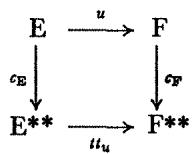
\includegraphics[keepaspectratio]{images/part002_cca49df6.jpg}}

是可交换的，这直接从定义和给出线性映射转置的公式(15)得出。

命题13. 若E是自由模（相应地，具有有限基的自由模），则典范映射 \(c_{E}:E \rightarrow E^{**}\) 是单射（相应地，双射）。

设 \((e_t)_{t \in \mathbb{T}}\) 是 \(\mathbf{E}\) 的一组基，并设 \((e_t^*)\) 为相应的坐标形式的族；根据定义，如果 \(x \in \mathbf{E}\) 满足 \(\tilde{x} = 0\) ，则 \(\langle x, e_t^* \rangle = 0\) 对所有 \(t \in \mathbb{T}\) 成立，换言之，即 \(x\) 的所有坐标均为零，因此 \(x = 0\) 。进一步假设 \(\mathbf{T}\) 是有限的；由于 \(\langle \tilde{e}_t, e_{t'}^* \rangle = \delta_{tt'}\) ， \((\tilde{e}_t)\) 是 \((e_t^*)\) 在 \(\mathbf{E}^{**}\) 中的对偶基，并且，由于 \(c_{\mathbf{E}}\) 把 \(\mathbf{E}\) 的一个基变换为 \(\mathbf{E}^{**}\) 的一个基， \(c_{\mathbf{E}}\) 是双射（§ 1，第 11 号，命题 17 的推论 3）。我们还证明了：

推论1. 设E是具有有限基的自由A-模；对于E的每个基 \((e_t)\) ， \((c_{\mathbf{E}}(e_t))\) 是 \((e_t^*)\) （E*的、与 \((e_t)\) 对偶的基）的对偶基。

在这种情况下，称 \((e_t)\) 和 \((e_t^*)\) 是彼此的对偶基。

推论2. 若E是具有有限基的自由A-模，则 \(\mathbf{E}^*\) 的每个有限基都是 \(\mathbf{E}\) 的某个基的对偶基。

只需考虑E**中给定基的对偶基，并将E典范地等同于E**即可。

推论3. 设E、F为两个均具有有限基的A-模，E（相应地，F）被典范地等同于其双重对偶E**（相应地，F**）。则对每个线性映射 \(u: \mathbf{E} \to \mathbf{F}\) ， \(^{tt}u = u\) 。

这直接从图表(27)的交换性得出。

推论4. 若P是投射模（相应地，有限生成投射模），则典范映射 \(c_{\mathbf{P}}: \mathbf{P} \to \mathbf{P}^{**}\) 是单射（相应地，双射）。

我们使用以下引理：

引理1. 设M、N是A-模E中的两个互补子模，i: M → E，j: N → E为典范单射。则图表

\begin{enumerate}
\def\labelenumi{(\arabic{enumi})}
\setcounter{enumi}{27}
\tightlist
\item
\end{enumerate}

\pandocbounded{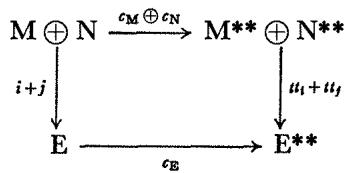
\includegraphics[keepaspectratio]{images/part002_690a791a.jpg}}

是交换的。

根据定义，对于 \(x \in \mathbf{M}\) , \(y \in \mathbf{N}\) , \(z^{*} \in \mathbf{E}^{*}\) ,

\[
\begin{array}{r l} \langle c _ {\mathrm{E}} (i (x) + j (y)), z ^ {*} \rangle & = \langle i (x) + j (y), z ^ {*} \rangle \\ & = \langle i (x), z ^ {*} \rangle + \langle j (y), z ^ {*} \rangle \\ & = \langle x, ^ {t} i (z ^ {*}) \rangle + \langle y, ^ {t} j (z ^ {*}) \rangle \\ & = \langle c _ {\mathrm{M}} (x), ^ {t} i (z ^ {*}) \rangle + \langle c _ {\mathrm{N}} (y), ^ {t} j (z ^ {*}) \rangle \\ & = \langle^ {t t} i (c _ {\mathrm{M}} (x)) + ^ {t t} j (c _ {\mathrm{N}} (y)), z ^ {*} \rangle . \end{array}
\]

既然如此，若E是自由模（相应地，具有有限基的自由模）， \(c_{E}\) 是单射（相应地，双射）；另一方面，由第6号、命题10可知， \(^{tt}i \oplus ^{tt}j\) 是双射的；图表(28)的交换性因此蕴含 \(c_{M} \oplus c_{N}\) 是单射（相应地，双射），因此 \(c_{M}\) 和 \(c_{N}\) （§1，第6号，命题7的推论1）亦然；考虑到第2号命题4，即得出推论。

\subsection{线性方程}

设 E、F 为两个 A-模。形如 \(u(x) = y_{0}\) 的每个方程（其中 \(u: E \to F\) 是一个给定的线性映射， \(y_{0}\) 是F的一个给定元素，而未知量x满足其取值在E中的条件）称为线性方程； \(y_{0}\) 称为方程的右端；如果 \(y_{0} = 0\) ，则方程称为齐次线性方程。

每个元素 \(x_{0} \in E\) ，若它满足 \(u(x_{0}) = y_{0}\) ，则称为线性方程 \(u(x) = y_{0}\) 的解。†

通常粗略地说，如果一个问题的求解等价于确定某个线性方程的解，那么这个问题就是线性的。

给定线性方程 \(u(x) = y_{0}\) ，方程 \(u(x) = 0\) 称为与 \(u(x) = y_{0}\) 相伴的齐次线性方程。

命题14. 若 \(x_{0}\) 是线性方程 \(u(x) = y_{0}\) 的一个解，则该方程的解集等于诸元素 \(x_{0} + z\) 的集合，其中 z 遍历相伴的齐次方程 \(u(x) = 0\) 的解集。

关系 \(u(x) = y_0\) 可以写成 \(u(x) = u(x_0)\) ，它等价于 \(u(x - x_0) = 0\) 。

换句话说，如果方程 \(u(x) = y_{0}\) 至少有一个解 \(x_{0}\) ，其解集就是集合 \(x_{0} + u^{-1}(0)\) ，它是由 u 的核 \(u^{-1}(0)\) 经平移得到的。注意， \(u^{-1}(0)\) 作为一个子模，永远不会是空的，因为它包含 0（称为齐次方程 \(u(x) = 0\) 的零解或平凡解）。

根据命题14，为使线性方程 \(u(x) = y_0\) 恰有一个解，必要且充分的是它至少有一个解，且 \(u^{-1}(0) = \{0\}\) （换句话说，即相伴的齐次方程没有非零解，或者说 \(u\) 是单射）；在这种情况下，对所有 \(y \in F\) ，方程 \(u(x) = y\) 至多有一个解。

命题15. 设 \(u\) 是模 \(\mathbf{E}\) 到模 \(\mathbf{F}\) 的一个线性映射。若方程 \(u(x) = y_0\) 至少有一个解，则 \(y_0\) 正交于 \(^t u\) 的核。

说 \(u(x) = y_{0}\) 有解意味着 \(y_{0} \in u(\mathbf{E})\) ，且该命题由第5号命题8的推论得出。

注意，命题15所给出的、方程 \(u(x) = y_{0}\) 有解的必要判据，当A是域时是充分的（§7，第6号，命题12），但一般不然（习题10）。

注记。(1) 设E是一个A-模， \((\mathbf{F}_{i})_{i\in I}\) 是一族A-模，并且对所有 \(i\in I\) ，设 \(u_{i}:E\to F_{i}\) 是一个线性映射。每个线性方程组

\[
u _ {i} (x) = y _ {i} \quad (i \in I)\tag{29}
\]

其中 \(y_{i} \in \mathbf{F}_{i}\) 是给定的，等价于单个线性方程 \(u(x) = y\) ，其中 \(u\) 是映射 \(x \mapsto (u_{i}(x))\) （从 \(\mathbf{E}\) 到 \(\mathbf{F} = \prod_{i \in I} \mathbf{F}_{i}\) ），而 \(y = (y_{i})\) 。方程组(29)称为齐次的，如果 \(y_{i} = 0\) 对所有 \(i \in I\) 成立。

\begin{enumerate}
\def\labelenumi{(\arabic{enumi})}
\setcounter{enumi}{1}
\tightlist
\item
  假设E有一个基 \((a_{\lambda})_{\lambda \in L}\) ；如果设 \(u(a_{\lambda}) = b_{\lambda}\) 对所有 \(\lambda \in L\) 成立，那么说 \(x = \sum_{\lambda \in L} \xi_{\lambda} a_{\lambda}\) 满足方程 \(u(x) = y_0\) ，就等价于说A中元素的（有限支撑的）族 \((\xi_{\lambda})_{\lambda \in L}\) 满足关系
\end{enumerate}

\[
\sum_ {\lambda \in L} \xi_ {\lambda} b _ {\lambda} = y _ {0}.\tag{30}
\]

反之，寻找A中元素的满足(30)的有限支撑的族 \((\xi_{\lambda})_{\lambda \in L}\) ，等价于求解线性方程 \(u(x) = y_0\) ，其中 \(u\) 是从 E 到 F 的唯一的线性映射，使得 \(u(a_{\lambda}) = b_{\lambda}\) 对所有 \(\lambda \in L\) 成立（§1，第 11 号，命题 17 的推论 3）。

\begin{enumerate}
\def\labelenumi{(\arabic{enumi})}
\setcounter{enumi}{2}
\tightlist
\item
  线性方程 \(u(x) = y_0\) 称为标量的，当 \(F = A_s\) ，从而 \(u\) 是 \(E\) 上的线性形式且 \(y_0\) 是标量时。若 \(E\) 有一组基 \((a_\lambda)_{\lambda \in L}\) ，则由注记（2）可知，这样的方程也可写成
\end{enumerate}

\[
\sum_ {\lambda \in L} \xi_ {\lambda} \alpha_ {\lambda} = y _ {0} \in A\tag{31}
\]

其中标量族 \((\alpha_{\lambda})\) 是任意的，并且约定该族 \((\xi_{\lambda})\) 必须具有有限支撑。一般地，标量线性方程组

\[
\sum_ {\lambda \in L} \xi_ {\lambda} \alpha_ {\lambda i} = \eta_ {i} \quad (i \in I)\tag{32}
\]

其中 \(\alpha_{\lambda i} \in A\) 且 \(\eta_i \in A\) ，其（A中的）解指的是一个有限支撑的族 \((\xi_\lambda)_{\lambda \in L}\) （由 \(A\) 中的元素组成），且满足(32)； \(\alpha_{\lambda i}\) 称为方程组的系数， \(\eta_i\) 称为右端项。这样的方程组的求解等价于方程 \(u(x) = y\) ，其中 \(y = (\eta_i)\) ，而 \(u: A_s^{(L)} \to A_s^I\) 是线性映射

\[
\left(\xi_ {\lambda}\right) \mapsto \left(\sum_ {\lambda \in L} \xi_ {\lambda} \alpha_ {\lambda i}\right).
\]

\begin{enumerate}
\def\labelenumi{(\arabic{enumi})}
\setcounter{enumi}{3}
\tightlist
\item
  线性方程组(32)在需要避免混淆时也称为左标量线性方程组。一个方程组
\end{enumerate}

\[
\sum_ {\lambda \in L} \alpha_ {\lambda i} \xi_ {\lambda} = \eta_ {i} \quad (i \in I)\tag{33}
\]

同样称为右标量线性方程组；把 \(\xi_{\lambda}, \eta_{i}\) 和 \(\alpha_{\lambda i}\) 视为属于A的相反环 A \(^{0}\) ，这样的方程组便可立即转化为方程组(32)。

\section{张量积}

\subsection{两个模的张量积}

设 \(G_{1}, G_{2}\) 为两个 Z-模；从集合 \(G = G_{1} \times G_{2}\) 到某个 Z-模的映射 u 称为双加性的（或 Z-双线性的），如果 \(u(x_{1}, x_{2})\) 关于 \(x_{1}\) 和关于 \(x_{2}\) 都是“加性的”；确切地说，这意味着，对于 \(x_{1}, y_{1}\) 在 \(G_{1}, x_{2}, y_{2}\) 在 \(G_{2}\) ，

\[
\begin{array}{l} u (x _ {1} + y _ {1}, x _ {2}) = u (x _ {1}, x _ {2}) + u (y _ {1}, x _ {2}) \\ u (x _ {1}, x _ {2} + y _ {2}) = u (x _ {1}, x _ {2}) + u (x _ {1}, y _ {2}). \end{array}
\]

注意这特别蕴含 \(u(0, x_2) = u(x_1, 0) = 0\) 对所有 \(x_1 \in \mathbf{G}_1, x_2 \in \mathbf{G}_2\) 成立。

设 A 为一个环，E 为一个右 A-模，F 为一个左 A-模。我们将考虑如下泛映射问题（集合论，IV，§ 3，第 1 号），其中 \(\Sigma\) 为 Z-模结构的类（此时态射即为 Z-线性映射，换言之，加法群同态），而 \(\alpha\) -映射是映射 \(f\) （从 E \(\times\) F 到某个 Z-模 G ），它们是 Z-双线性的，并且进一步满足：对所有 \(x \in \mathbf{E}\) , \(y \in \mathbf{F}\) 和 \(\lambda \in \mathbf{A}\)

\[
f (x \lambda , y) = f (x, \lambda y).\tag{1}
\]

我们证明该问题有解。为此，我们考虑Z-模 \(C = \mathbf{Z}^{(E \times F)}\) ，即由 \(E \times F\) 的元素以Z中为系数的形式线性组合所构成的Z-模（§1，第11号），其一组基可视为由有序对 \((x, y)\) （其中 \(x \in E\) ， \(y \in F\) ）组成。设D为C的子Z-模，由以下类型的元素生成：

\[
\left\{ \begin{array}{l} (x _ {1} + x _ {2}, y) - (x _ {1}, y) - (x _ {2}, y) \\ (x, y _ {1} + y _ {2}) - (x, y _ {1}) - (x, y _ {2}) \\ (x \lambda , y) - (x, \lambda y) \end{array} \right.\tag{2}
\]

其中 \(x, x_{1}, x_{2}\) 属于E， \(y, y_{1}, y_{2}\) 属于F，且 \(\lambda\) 属于A。

定义1. 右A-模E与左A-模F的张量积，记为 \(\mathbf{E} \otimes_{\mathbf{A}} \mathbf{F}\) 或 \(\mathbf{E} \otimes_{\mathbf{A}} \mathbf{F}\) （若不致引起混淆，也简记为 \(\mathbf{E} \otimes \mathbf{F}\) ），指的是商 \(\mathbf{Z}\) -模 C/D（即 \(\mathbf{Z}\) -模 C——由 \(\mathbf{E} \times \mathbf{F}\) 的元素以 \(\mathbf{Z}\) 中为系数的形式线性组合构成——除以由 (2) 中某一类型的元素所生成的子模 \(\mathbf{D}\) 而得的商）。对于 \(x \in \mathbf{E}\) 和 \(y \in \mathbf{F}\) ， \(\mathbf{E} \otimes_{\mathbf{A}} \mathbf{F}\) 中作为元素 \((x, y)\) （属于 \(\mathbf{C} = \mathbf{Z}^{(\mathbf{E} \times \mathbf{F})}\) ）的典范像的那个元素记为 \(x \otimes y\) ，并称为 \(x\) 与 \(y\) 的张量积。

映射 \((x,y)\mapsto x\otimes y\) 于 \(\mathbf{E}\times \mathbf{F}\) 到 \(\mathbf{E}\otimes_{\mathbf{A}}\mathbf{F}\) 称为典范的。它是一个满足条件(1)的Z-双线性映射。

我们证明张量积 \(E \otimes_{A} F\) 并且上述典范映射构成了先前提出的泛映射问题的一个解。确切地说：

命题1. (a) 设 \(g\) 是一个 \(\mathbf{Z}\) -线性映射（从 \(\mathbf{E} \otimes_{\mathbf{A}} \mathbf{F}\) 到某个 \(\mathbf{Z}\) -模 \(\mathbf{G}\) ）。映射 \((x, y) \mapsto f(x, y) = g(x \otimes y)\) （从 \(\mathbf{E} \times \mathbf{F}\) 到 \(\mathbf{G}\) ）是 \(\mathbf{Z}\) -双线性的，且满足条件(1)。

\begin{enumerate}
\def\labelenumi{(\alph{enumi})}
\setcounter{enumi}{1}
\tightlist
\item
  反之，设 \(f\) 是一个 \(\mathbf{Z}\) -双线性映射（从 \(\mathbf{E} \times \mathbf{F}\) 到某个 \(\mathbf{Z}\) -模 \(\mathbf{G}\) ），它满足条件(1)。则存在且仅存在一个 \(\mathbf{Z}\) -线性映射 \(g\) （从 \(\mathbf{E} \otimes_{\mathbf{A}} \mathbf{F}\) 到 \(\mathbf{G}\) ），使得 \(f(x,y) = g(x \otimes y)\) 对所有 \(x \in \mathbf{E}, y \in \mathbf{F}\) 成立。
\end{enumerate}

若 \(\phi\) 表示 \(\mathbf{E} \times \mathbf{F}\) 到 \(\mathbf{E} \otimes_{\mathbf{A}} \mathbf{F}\) 的典范映射，则 \(f = g \circ \phi\) ；由此得(a)。为证明(b)，我们注意到，在定义1的记号下， \(f\) 可延拓为一个 \(\mathbf{Z}\) -线性映射 \(\bar{f}\) （从 \(\mathbf{C}\) 到 \(\mathbf{G}\) ）（ \(\S 1\) ，第11号，命题17）。根据关系式(1)， \(\bar{f}\) 在 \(\mathbf{C}\) 的 (2) 中某一类型的所有元素上均为零，从而在 \(\mathbf{D}\) 上为零。因此存在一个 \(\mathbf{Z}\) -线性映射 \(g\) （从 \(\mathbf{C} / \mathbf{D} = \mathbf{E} \otimes_{\mathbf{A}} \mathbf{F}\) 到 \(\mathbf{G}\) ），使得 \(\bar{f} = g \circ \psi\) ，其中 \(\psi: \mathbf{C} \to \mathbf{C} / \mathbf{D}\) 是典范同态（ \(\S 1\) ，第8号，注记）。 \(g\) 的唯一性是直接的，因为 \(\mathbf{E} \otimes_{\mathbf{A}} \mathbf{F}\) 作为 \(\mathbf{Z}\) -模由形如 \(x \otimes y\) 的元素生成。

命题1定义了一个典范同构，它把E × F到G的、满足条件(1)的Z-双线性映射f所成的Z-模映到Z-模Hom \(_{Z}\) (E ⊗A F, G)上。

当 A = Z 时，条件 (1) 对每个 Z-双线性映射 f 自动满足，且 C 的子模 D 已由 (2) 中前两类元素生成。

现在我们回到一般情形，并且 \(E'\) 和 \(F'\) 分别表示E和F的底层Z-模，上述注记和定义1立即表明该Z-模 \(E \otimes_{A} F\) 可以典范地等同于 Z-模 \(E' \otimes_{Z} F'\) 的商模，该商模由形如 \((x\lambda) \otimes y - x \otimes (\lambda y)\) 的元素生成的子 Z-模所决定，其中 x 遍历 E，y 遍历 F，且 \(\lambda\) 遍历A。

推论1. 设H是一个Z-模，且 \(h:E \times F \rightarrow H\) 是一个满足条件(1)的Z-双线性映射，使得H由 \(h(E \times F)\) 生成。假设对于每个Z-模G以及每个从 \(E \times F\) 到G的满足(1)的Z-双线性映射f，

都存在一个Z-线性映射 \(g:H \to G\) ，使得 \(f = g \circ h\) 。那么，若 \(\phi\) 表示 \(E \times F\) 到 \(E \otimes_{A} F\) 的典范映射，则存在且仅存在一个同构 \(\theta\) （从 \(E \otimes_{A} F\) 到H上），使得 \(h = \theta \circ \phi\) 。

假设 \(h(\mathbf{E} \times \mathbf{F})\) 生成 H 蕴含了 g 的唯一性；该推论不过是泛映射问题解的一般唯一性性质（集合论，IV，§ 3，第 1 号）。

推论2. 设 \(\mathbf{E}^0\) （相应地 \(\mathbf{F}^0\) ）表示模 \(\mathbf{E}\) （相应地 \(\mathbf{F}\) ）被视为相反环 \(\mathbf{A}^0\) 上的左（相应地，右）模；则存在且仅存在一个 \(\mathbf{Z}\) -模同构 \(\sigma: \mathbf{E} \otimes_{\mathbf{A}} \mathbf{F} \to \mathbf{F}^0 \otimes_{\mathbf{A}^0} \mathbf{E}^0\) ，使得 \(\sigma(x \otimes y) = y \otimes x\) 对所有 \(x \in \mathbf{E}\) 和 \(y \in \mathbf{F}\) 成立（张量积的“交换性”）。

根据 \(A^{0}\) -模结构（在 \(E^{0}\) 和 \(F^{0}\) 上）的定义，映射 \((x,y)\mapsto y\otimes x\) （从 \(E\times F\) 到 \(F^{0}\otimes_{A^{0}}E^{0}\) ）是Z-双线性的且满足条件(1)，由此得到Z-线性映射 \(\sigma\) 的存在性和唯一性。类似地，可定义一个Z-线性映射 \(\tau:F^{0}\otimes_{A^{0}}E^{0}\to E\otimes_{A}F\) 使得 \(\tau(y\otimes x)=x\otimes y\) ，并且显然 \(\sigma\) 和 \(\tau\) 是互逆的同构。

注记. 非零模的张量积可能为零：例如，取两个Z-模 E = Z/2Z 和 F = Z/3Z，则对所有 \(x \in E\) 和 \(y \in F\) 都有 2x = 0 和 3y = 0；因此，在 E \(\otimes_{\mathbf{Z}} F\) 中，

\[
x \otimes y = 3 (x \otimes y) - 2 (x \otimes y) = x \otimes (3 y) - (2 x) \otimes y = 0
\]

对所有 \(x\) 和 \(y\) 成立（参见第6号，命题6的推论4）。

\subsection{两个线性映射的张量积}

设A是一个环，E、E'是两个右A-模，F、F'是两个左A-模，且 \(u: E \rightarrow E'\) 和 \(v: F \rightarrow F'\) 是两个A-线性映射。容易验证，映射

\[
(x, y) \mapsto u (x) \otimes v (y)
\]

（从 \(\mathbf{E} \times \mathbf{F}\) 到 \(\mathbf{E}' \otimes_{\mathbf{A}} \mathbf{F}'\) ）是 \(\mathbf{Z}\) -双线性的，且满足第1号的条件(1)。因此，根据第1号命题1，存在且仅存在一个 \(\mathbf{Z}\) -线性映射 \(w: \mathbf{E} \otimes_{\mathbf{A}} \mathbf{F} \to \mathbf{E}' \otimes_{\mathbf{A}} \mathbf{F}'\) ，使得

\[
w (x \otimes y) = u (x) \otimes v (y)\tag{3}
\]

对于 \(x \in \mathbf{E}\) ， \(y \in \mathbf{F}\) 。此映射记作 \(u \otimes v\) （当不致引起混淆时），并称为线性映射 \(u\) 与 \(v\) 的张量积。

由(3)立即得出 \((u, v) \mapsto u \otimes v\) 是一个Z-双线性映射，称为典范映射

\[
\operatorname{Hom} _ {\mathbf {A}} (\mathrm{E}, \mathrm{E} ^ {\prime}) \times \operatorname{Hom} _ {\mathbf {A}} (\mathrm{F}, \mathrm{F} ^ {\prime}) \rightarrow \operatorname{Hom} _ {\mathbf {Z}} (\mathrm{E} \otimes_ {\mathbf {A}} \mathrm{F}, \mathrm{E} ^ {\prime} \otimes_ {\mathbf {A}} \mathrm{F} ^ {\prime}).
\]

根据第1号命题1，与之对应的是一个 \(\mathbf{Z}\) -线性映射，称为典范映射

\[
\operatorname{Hom} _ {\mathbf {A}} (\mathrm{E}, \mathrm{E} ^ {\prime}) \otimes_ {\mathbf {Z}} \operatorname{Hom} _ {\mathbf {A}} (\mathrm{F}, \mathrm{F} ^ {\prime}) \rightarrow \operatorname{Hom} _ {\mathbf {Z}} (\mathrm{E} \otimes_ {\mathbf {A}} \mathrm{F}, \mathrm{E} ^ {\prime} \otimes_ {\mathbf {A}} \mathrm{F} ^ {\prime})\tag{4}
\]

它把张量积的每个元素 \(u \otimes v\) 对应到线性映射 \(u \otimes v: \mathbf{E} \otimes_{\mathbf{A}} \mathbf{F} \to \mathbf{E}' \otimes_{\mathbf{A}} \mathbf{F}'\) 。注意，典范映射(4)不一定是单射的，也不一定是满射的。因此记号 \(u \otimes v\) 可能引起混淆，须由上下文指明它表示的是张量积的元素还是线性映射。

此外，设 \(\mathbf{E}''\) 是一个右A-模， \(\mathbf{F}''\) 是一个左A-模，且 \(u':\mathbf{E}'\to\mathbf{E}''\) , \(v':\mathbf{F}'\to\mathbf{F}''\) 是A-线性映射；由(3)得出

\[
\left(u ^ {\prime} \circ u\right) \otimes \left(v ^ {\prime} \circ v\right) = \left(u ^ {\prime} \otimes v ^ {\prime}\right) \circ (u \otimes v).\tag{5}
\]
